\documentclass[a4paper,11pt]{report}

% Packages
\usepackage[utf8]{inputenc}
\usepackage[T1]{fontenc}
\usepackage[ngerman]{babel} % For German language
\usepackage{graphicx}
\usepackage{amsmath}
\usepackage{amsfonts}
\usepackage{amssymb}
\usepackage{hyperref}
\usepackage{listings} % For code listings
\usepackage{setspace} % For line spacing
\usepackage{geometry} % For setting margins
\usepackage{titlesec} % For customizing title formats
\usepackage{chngcntr} % For changing counter settings
\usepackage{fancyhdr} % For custom headers and footers
\usepackage[style=ieee,backend=biber,url=true,citestyle=numeric-comp]{biblatex}
\addbibresource{references.bib}
% Remove empty parenthesis if no date specified 
\DeclareFieldFormat{parens}{%
  \iffieldundef{year}{}{\mkbibparens{#1}}%
}
\DeclareFieldFormat{date}{%
  \iffieldundef{year}{n.d.}{#1}%
}

\usepackage{float}
\usepackage{titling}
\usepackage{svg}
\usepackage{pdfpages}
\usepackage{array}
\usepackage{acro}
\usepackage{csquotes}
\usepackage{url}
\usepackage{breakurl}
\usepackage[export]{adjustbox}
\usepackage{booktabs}
\usepackage{longtable}
%\newcolumntype{P}[1]{>{\raggedright\arraybackslash}p{#1}}
\usepackage{tabularx}  % Automatically adjusts table width
\usepackage{hyperref}
\usepackage{subcaption}
\usepackage{xcolor}
\usepackage{siunitx}
\usepackage{listings}

\lstdefinelanguage{json}{
    morestring=[b]",
    morecomment=[l]{//},
    morekeywords={true, false, null},
    sensitive=false,
}

\lstset{
    language=json,
    backgroundcolor=\color{gray!10},
    basicstyle=\ttfamily\small,
    keywordstyle=\color{blue},
    stringstyle=\color{orange},
    commentstyle=\color{gray},
    showstringspaces=false,
    breaklines=true
}

% Margins
\geometry{
    left=3cm,
    right=2.5cm,
    top=2.5cm,
    bottom=2.5cm
}

% Line spacing
\onehalfspacing % 1.5 line spacing, you can use \singlespacing for single line spacing

% Remove ident before newline
\setlength{\parindent}{0pt}

% Decimal numbering without "Kapitel" prefix
\titleformat{\chapter}[block]
  {\normalfont\huge\bfseries}{\thechapter.}{20pt}{\Large}
\titleformat{\section}
  {\normalfont\Large\bfseries}{\thesection.}{1em}{}
\titleformat{\subsection}
  {\normalfont\large\bfseries}{\thesubsection.}{1em}{}
\titleformat{\subsubsection}
  {\normalfont\normalsize\bfseries}{\thesubsubsection.}{1em}{}

% Custom headers
\pagestyle{fancy}
\fancyhf{}
\fancyhead[L]{\leftmark}    % Left side of the header
\fancyfoot[C]{\thepage}     % Mid side of the footer

% Redefine \leftmark to show only the chapter number and title
\renewcommand{\chaptermark}[1]{\markboth{\thechapter.\ #1}{}}

% \input{acronyms.tex}

\begin{document}

% Title Page
\begin{titlepage}
    \begin{flushleft}
        
\includegraphics[width=.6\textwidth]{./images/oth.png}
    \end{flushleft}

    \vspace*{2cm}

    \centering
    {\scshape\Large Datenverarbeitung in der Technik \par}
    \vspace{0.5cm}
    {\scshape Sommersemester 2025 \par}
    \vspace{0.5cm}
    {\huge\bfseries Projektbericht \par}
    \vspace{3cm}

    \begin{flushleft}
        \large
        \textbf{Teammitglieder:} \\
        \vspace{0.5cm}

        Fabian Becker\hfill\makebox[8cm]{\hrulefill} \\[0.5cm]
        Jendrik Jürgens\hfill\makebox[8cm]{\hrulefill} \\[0.5cm]
        Nicolas Koch\hfill\makebox[8cm]{\hrulefill} \\[0.5cm]
        Michael Specht\hfill\makebox[8cm]{\hrulefill} \\[0.5cm]
        Jonathan Wohlrab\hfill\makebox[8cm]{\hrulefill} \\[1cm]

        \textbf{Betreuung:} \\
        Dr. Alexander Metzner, Matthias Altmann \\
        \vspace{0.5cm}

        \textbf{Abgabedatum:} \\
        15.07.2025 \\
    \end{flushleft}

    \vfill
    \centering
    {\large \today\par}
\end{titlepage}


% Table of Contents
\tableofcontents
\newpage

% Main Content
\chapter{Stromversorgung}

\section{Analyse des Aufbaus und der Komponenten des vorherigen Projekts (Koch)}

Zu Beginn wurde die bestehende Stromversorgung und die dafür genutzten Komponenten eines früheren Semesterprojekts analysiert, um anhand dessen bestimmen zu können, welche Teile wiederverwendet werden können, sowie ob das gegebene Layout in etwa für das eigene Projekt genutzt werden kann.

Essentiell bestand die Stromversorgung aus zwei Step-Down-Wandlern, die aus einer Eingangsspannung eine 8V und eine 5V Ausgangsspannung erzeugten, was ebenfalls für unser eigenes Projekt benötigt wird. Außerdem wurden zwei Verteiler genutzt, um die Spannungen auf die verschiedenen Sensoren und Aktoren zu verteilen.
Das vorhandene Layout auf dem Lochrastergerüst war für uns jedoch nicht geeignet, da wir einen übersichtlicheren Aufbau und ein sinnvolles Color-Coding der Kabel für die verschiedenen Anschlüsse und für einen besseren Überblick anstrebten.

\section{Aufbau der eigenen Stromversorgung (Koch)}
Nachdem die vorhandenen Teile analysiert wurden, wurde die Entscheidung getroffen nur die Step-Down-Wandler, da der Rest nicht relevant für unser Projekt war. Lediglich die Verteiler brauchten wir auch, mussten allerdings ersetzt werden, da die Schraubverbindungen kaputt waren.
Die Step-Down-Wandler waren so aufgebaut, dass ein Modul die Eingangsspannung erhielt und am Ausgang ein selbstangefertigtes Y-Kabel hatte, welches dann jeweils in einen Verteiler und in den anderen Step-Down-Wandler ging.
Diese Kombination sollte auch so für unser Projekt übernommen werden, allerdings mussten dafür die Kabel erneuert werden, da die alten Kabel nicht dem geplanten Color-Coding entsprachen und zu kurz waren. Dabei stellte sich heraus, dass der entstandene Durchmesser, durch die Kombination aus zwei Kabeln zu einem Y-Kabel, zu groß war, um in die Steckverbindung zu passen.
Aus diesem Grund entstand das alternative Konzept die ausgehenden Kabel des ersten Step-Down-Wandlers mit dem ersten Verteiler zu verbinden. Das war vor allem dadurch leicht realisierbar, da jeder Verteiler 12 Ports besitzt und 8V lediglich für die Motoren zum fahren benötigt werden. Somit konnte eine Verbindung vom 8V-Verteiler zum zweiten Step-Down-Wanlder hergestellt werden ohne dabei die Steckverbindungen zu beschädigen.
\newpage
Das Color-Coding der Kabel wurde wie folgt eingeführt:
\begin{itemize}
    \item \textbf{Rot:} Versorgungsspannung
    \item \textbf{Schwarz:} Masse
    \item \textbf{Weiß:} PWM-Verbindung für Motoren
    \item \textbf{Gelb:} Direction Pin für Motoren
\end{itemize}
Des Weiteren wurde darauf geachtet, dass die Kabel so kurz wie möglich gehalten werden und wenn möglich unter der Platte verlegt werden, um eine bessere Übersicht zu gewährleisten.

Als Eingangsspannung wurde zu Beginn ein 6V-Batterieverbund genutzt, der im Laufe des Projekts durch einen 12V-Batterieverbund ausgetauscht wurde, da beim Testing der Motortreiber festgestellt wurde, dass die Motoren eine höhere Spannung benötigen, um korrekt zu funktionieren. Außerdem wurde versucht den Raspberry Pi 5 über den 5V-Verteiler zu versorgen, was jedoch nicht funktionierte, da die Stromstärke zu niedrig war, wenn der Pi aufwendigere Aufgaben erledigen musste. Aus diesem Grund wurde eine Powerbank genutzt, die den Pi mit Strom versorgt und somit die 5V-Verteilung entlastet.

Der Gesamtaufbau der Stromversorgung sieht dabei wie folgt aus:
\begin{itemize}
    \item \textbf{12V-Batterieverbund:}
    \begin{itemize}
        \item Step-Down-Wandler (8V) $\rightarrow$ 8V-Verteiler
        \begin{itemize}
            \item 2 PWM Boards für Motoren
            \item Step-Down-Wandler (5V) $\rightarrow$ 5V-Verteiler
            \begin{itemize}
                \item ESP32
                \item 2 PWM Boards für die Flywheel Motoren
                \item Servo-Motor für die Geschützplattform
                \item Servo-Motor für den Geschützarm
            \end{itemize}
        \end{itemize}
    \end{itemize}
    
    \item \textbf{Powerbank:}
    \begin{itemize}
        \item Raspberry Pi 5
        \begin{itemize}
            \item Pi-Camera
            \item MPU6050 Gyrosensor
            \item SRF02 Ultraschallsensor
        \end{itemize}
    \end{itemize}
\end{itemize}

\chapter{CAD-Konstruktion}

\section{Setup und Einarbeitung (Becker, Specht)}

Zu Beginn des Projekts wurde in Abstimmung mit Fabian Becker sowie im Austausch mit Andreas Wittmann (Studienkollege) entschieden, FreeCAD als CAD-Software zu verwenden. Der Grund hierfür war die einfache Kollaboration innerhalb der Projektgruppe sowie der unkomplizierte Erfahrungsaustausch mit der Arbeitsgruppe um A. Wittmann. Andere Softwarelösungen wie OnShape wurden diskutiert, aufgrund der Komplexität und der damit verbundenen Einarbeitungszeit im Hinblick auf die Projektlaufzeit jedoch verworfen. FreeCAD ist zudem eine Open-Source-Software, die neben Fedora auch auf Debian-Systemen lauffähig ist. So konnte die Software problemlos auf den Arbeitsrechnern der Teammitglieder installiert werden.

Grundsätzlich stützt sich die Konstruktion auf vorhandene STL-Vorlagen. Ein Beispielprojekt aus dem Internet diente als Grundlage für die Arbeit.

\section{Geschützarm Version 1 (Specht) \label{sec:cad_gunarm_v1}}

Bevor mit der Konstruktion begonne wurde, wurde im Team besprochen, welche Komponenten nötig sind, um die Position des Flugobjekts eindeutig zu bestimmen. Die Wahl fiel auf folgende Komponenten, die aus vorherigen Studienprojekten übernommen werden konnten:

\begin{itemize}
    \item GY-521 MPU-6050 3-Achsen-Gyroskop und Beschleunigungssensor
    \item SRF02 Ultraschall Entfernungssensor
    \item Raspberry Pi 5 Kamera Modul
    \item 2x 28BYJ-48 Schrittmotor
\end{itemize}

Ziel des ersten Entwurfs war es, diese kompakt auf dem Arm zu integrieren. Die angedachten Schrittmotoren wichen jedoch von der Vorlage aus dem Beispielprojekt ab, weshalb der Geschützarm von Grund auf neu konstruiert werden musste.

Alle Module sollten zentral über der Abschusseinrichtung platziert werden, um eine korrekte Berechnung der Flugbahn zu ermöglichen. Der Ultraschall-Sensor sollte dabei hochkant nach vorne gerichtet sein, um die Entfernung zum Ziel zu messen. Die Kamera sollte schräg nach oben gerichtet sein, um den Himmel zu überwachen. Der Beschleunigungssensor sollte liegend auf dem Arm montiert werden, um die Beschleunigung des Arms zu messen. Die Schrittmotoren mussten in einem geeigneten Abstand zueinander montiert werden, sodass die Flywheel-Konstruktion des Arms funktioniert. Letzteres konnte durch das Vermessen der Vorlage aus dem Beispielprojekt realisiert werden. Für die restlichen Anforderungen waren die korrekten Maße nötig. Für die Montage der Kamera konnte eine bereits 3D-gedruckte Halterung aus einer anderen Gruppe benutzt werden. Die Haltevorrichtung für den Beschleunigungssensor wurde aus einer STL-Vorlage übernommen und angepasst. Auch für die Schrittmotoren konnte auf ein Modell aus dem Internet zurückgegriffen werden, weshalb es nicht nötig war, die komplexe Geometrie eigenständig zu vermessen. Einzig die Maße für den Ultraschall-Sensor wurden recherchiert und durch Nachmessen validiert.

\begin{figure}[h]
    \centering

    \begin{subfigure}[b]{0.45\textwidth}
        \centering
        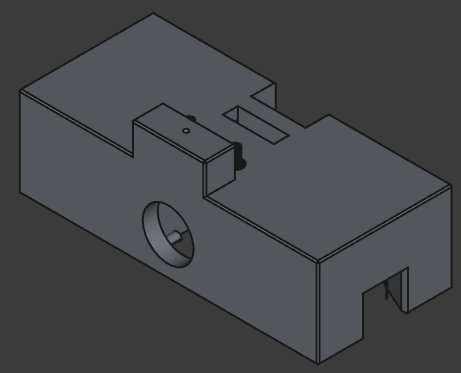
\includegraphics[width=\textwidth]{images/cad_gunarm_v1_front.jpg}
        \caption{Geschützarm Version 1 - Frontansicht}
    \end{subfigure}
    \hfill
    \begin{subfigure}[b]{0.45\textwidth}
        \centering
        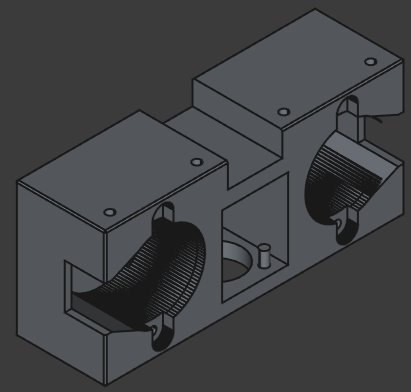
\includegraphics[width=\textwidth]{images/cad_gunarm_v1_back.jpg}
        \caption{Geschützarm Version 1 - Rückansicht}
    \end{subfigure}

    \caption{Geschützarm Version 1}
    \label{fig:gunarm_v1}
\end{figure}

Neben den eigentlichen Maßen der Komponenten war das Kabelmanagement ein wichtiges Thema. Alle Kabel sollten nach hinten am Magazin entlang geführt werden, um eine saubere Optik zu gewährleisten. Für Beschleunigungssensor und Kamera stellte dies kein Problem dar, da diese ganz oben angebracht sein sollten. Der Ultraschall-Sensor und die Schrittmotoren hingegen waren in das neukonstruierte Gehäuse integriert, sodass Aussparungen, wie in Abbildung~\ref{fig:gunarm_v1} zu sehen, angebracht werden mussten, um die Kabel aus dem Gehäuse herauszuführen.

Außerdem musste sichergestellt werden, dass der Geschützarm an das Magazin montiert werden kann. Hierzu wurden vom Kollegen Fabian Becker Montagepunkte am Magazin konstruiert, die mit dem Geschützarm verschraubt werden können.

\section{Geschützarm Version 2 (Specht)}

Im Laufe des Projektes wurde in Abstimmung mit Fabian Becker klar, dass die Schrittmotoren aufgrund zu geringer Leistung nicht für die Flywheel-Konstruktion geeignet sind. Daraufhin wurde sich für die originalen Motoren aus dem Beispielprojekt entschieden. Das hatte zur Folge, dass der Geschützarm neu konstruiert werden musste, da die Maße der neuen Motoren von den Alten abwichen. Aus diesem Grund wurde der Geschützarm der Vorlage als Basis genommen und die Grundidee der Version 1 beibehalten.

\begin{figure}[h]
    \centering

    \begin{subfigure}[b]{0.45\textwidth}
        \centering
        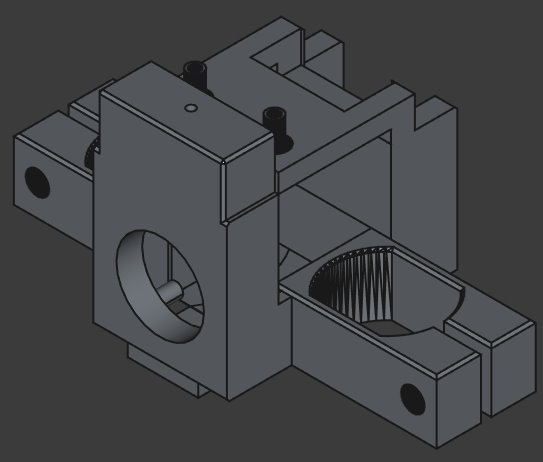
\includegraphics[width=\textwidth]{images/cad_gunarm_v2_front.jpg}
        \caption{Geschützarm Version 2 - Frontansicht}
    \end{subfigure}
    \hfill
    \begin{subfigure}[b]{0.45\textwidth}
        \centering
        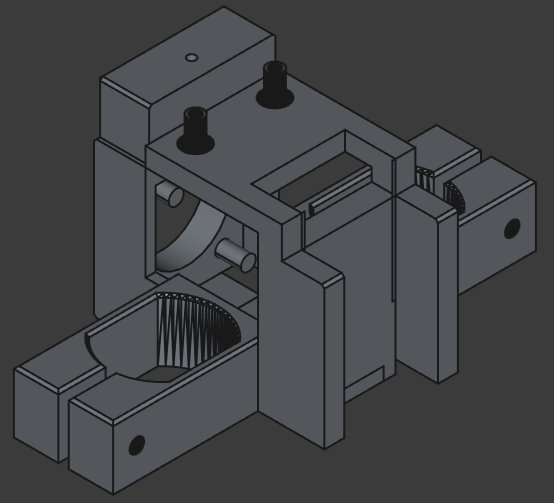
\includegraphics[width=\textwidth]{images/cad_gunarm_v2_back.jpg}
        \caption{Geschützarm Version 2 - Rückansicht}
    \end{subfigure}

    \caption{Geschützarm Version 2}
    \label{fig:gunarm_v2}
\end{figure}

Im Gegensatz zur Version 1 wird der Ultraschallsensor nun seitlich eingeführt anstatt von unten, siehe~\ref{fig:gunarm_v2}. Problematisch waren dabei die beschränkten Platzverhältnisse, da die Schrittmotoren näher am Kanonenrohr angebracht wurden als im vorherigen Entwurf. Außerdem wurden die zuvor angedachten Montagepunkte am Magazin wieder entfernt. Die Zusammenführung des Geschützarms mit dem Magazin erfolgte deshalb mittels Modellbaukleber.

\section{Montagehalterung Motortreiber (Specht)}

Für die ersten Funktionstests wurden die Pololu-Motoren provisorisch auf Kork-Schnipseln montiert. Dieses Vorgehen ermöglichte eine zügige Inbetriebnahme, jedoch erwies es sich hinsichtlich Stabilität und Sicherheit als unzureichend. Im Rahmen der Tests kam es zum Abrutschen eines Motors von der Korkunterlage, was zu einer kurzfristigen Wärmeentwicklung und Geruchsbildung führte. Glücklicherweise wurde eine Beschädigung der Hardware vermieden.

\begin{figure}[h]
    \centering

    \begin{subfigure}[b]{0.25\textwidth}
        \centering
        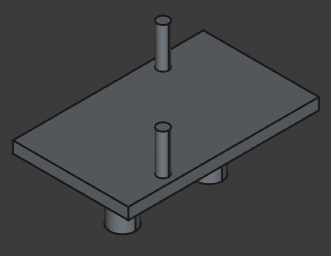
\includegraphics[width=\textwidth]{images/cad_polulu_front.png}
        \caption{Polulu - Draufsicht}
    \end{subfigure}
    \hspace{0.05\textwidth} % Adjust this value as needed
    \begin{subfigure}[b]{0.25\textwidth}
        \centering
        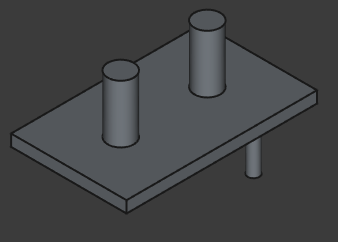
\includegraphics[width=\textwidth]{images/cad_polulu_back.png}
        \caption{Polulu - Bodensicht}
    \end{subfigure}

    \caption{Montagehalterung für Pololu-Motortreiber}
    \label{fig:pololu_mounting}
\end{figure}

Für die finale Abnahme wurde daher ein dauerhaftes und sicheres Montagesystem umgesetzt, das ein sauberes und zuverlässiges Setup gewährleistet. Wie in Abbildung~\ref{fig:pololu_mounting} zu sehen, kann die Halterung direkt auf der Montageplatte des Fahrzeugs geklippt werden.
\chapter{CAD-Konstruktion}

\section{Setup und Einarbeitung (Becker, Specht)}

Zu Beginn des Projekts wurde in Abstimmung mit Fabian Becker sowie im Austausch mit Andreas Wittmann (Studienkollege) entschieden, FreeCAD als CAD-Software zu verwenden. Der Grund hierfür war die einfache Kollaboration innerhalb der Projektgruppe sowie der unkomplizierte Erfahrungsaustausch mit der Arbeitsgruppe um A. Wittmann. Andere Softwarelösungen wie OnShape wurden diskutiert, aufgrund der Komplexität und der damit verbundenen Einarbeitungszeit im Hinblick auf die Projektlaufzeit jedoch verworfen. FreeCAD ist zudem eine Open-Source-Software, die neben Fedora auch auf Debian-Systemen lauffähig ist. So konnte die Software problemlos auf den Arbeitsrechnern der Teammitglieder installiert werden.

Grundsätzlich stützt sich die Konstruktion auf vorhandene STL-Vorlagen. Ein Beispielprojekt aus dem Internet diente als Grundlage für die Arbeit.

\section{Geschützarm Version 1 (Specht) \label{sec:cad_gunarm_v1}}

Bevor mit der Konstruktion begonne wurde, wurde im Team besprochen, welche Komponenten nötig sind, um die Position des Flugobjekts eindeutig zu bestimmen. Die Wahl fiel auf folgende Komponenten, die aus vorherigen Studienprojekten übernommen werden konnten:

\begin{itemize}
    \item GY-521 MPU-6050 3-Achsen-Gyroskop und Beschleunigungssensor
    \item SRF02 Ultraschall Entfernungssensor
    \item Raspberry Pi 5 Kamera Modul
    \item 2x 28BYJ-48 Schrittmotor
\end{itemize}

Ziel des ersten Entwurfs war es, diese kompakt auf dem Arm zu integrieren. Die angedachten Schrittmotoren wichen jedoch von der Vorlage aus dem Beispielprojekt ab, weshalb der Geschützarm von Grund auf neu konstruiert werden musste.

Alle Module sollten zentral über der Abschusseinrichtung platziert werden, um eine korrekte Berechnung der Flugbahn zu ermöglichen. Der Ultraschall-Sensor sollte dabei hochkant nach vorne gerichtet sein, um die Entfernung zum Ziel zu messen. Die Kamera sollte schräg nach oben gerichtet sein, um den Himmel zu überwachen. Der Beschleunigungssensor sollte liegend auf dem Arm montiert werden, um die Beschleunigung des Arms zu messen. Die Schrittmotoren mussten in einem geeigneten Abstand zueinander montiert werden, sodass die Flywheel-Konstruktion des Arms funktioniert. Letzteres konnte durch das Vermessen der Vorlage aus dem Beispielprojekt realisiert werden. Für die restlichen Anforderungen waren die korrekten Maße nötig. Für die Montage der Kamera konnte eine bereits 3D-gedruckte Halterung aus einer anderen Gruppe benutzt werden. Die Haltevorrichtung für den Beschleunigungssensor wurde aus einer STL-Vorlage übernommen und angepasst. Auch für die Schrittmotoren konnte auf ein Modell aus dem Internet zurückgegriffen werden, weshalb es nicht nötig war, die komplexe Geometrie eigenständig zu vermessen. Einzig die Maße für den Ultraschall-Sensor wurden recherchiert und durch Nachmessen validiert.

\begin{figure}[h]
    \centering

    \begin{subfigure}[b]{0.45\textwidth}
        \centering
        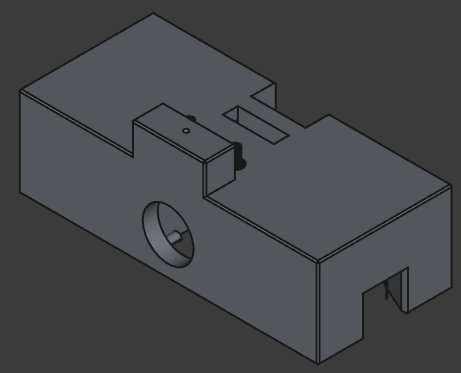
\includegraphics[width=\textwidth]{images/cad_gunarm_v1_front.jpg}
        \caption{Geschützarm Version 1 - Frontansicht}
    \end{subfigure}
    \hfill
    \begin{subfigure}[b]{0.45\textwidth}
        \centering
        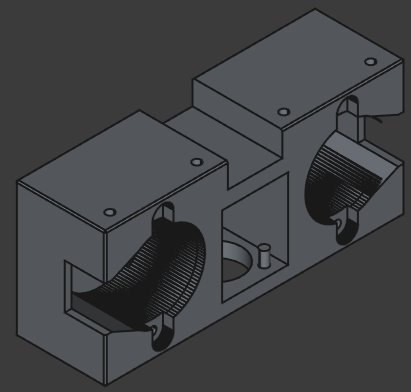
\includegraphics[width=\textwidth]{images/cad_gunarm_v1_back.jpg}
        \caption{Geschützarm Version 1 - Rückansicht}
    \end{subfigure}

    \caption{Geschützarm Version 1}
    \label{fig:gunarm_v1}
\end{figure}

Neben den eigentlichen Maßen der Komponenten war das Kabelmanagement ein wichtiges Thema. Alle Kabel sollten nach hinten am Magazin entlang geführt werden, um eine saubere Optik zu gewährleisten. Für Beschleunigungssensor und Kamera stellte dies kein Problem dar, da diese ganz oben angebracht sein sollten. Der Ultraschall-Sensor und die Schrittmotoren hingegen waren in das neukonstruierte Gehäuse integriert, sodass Aussparungen, wie in Abbildung~\ref{fig:gunarm_v1} zu sehen, angebracht werden mussten, um die Kabel aus dem Gehäuse herauszuführen.

Außerdem musste sichergestellt werden, dass der Geschützarm an das Magazin montiert werden kann. Hierzu wurden vom Kollegen Fabian Becker Montagepunkte am Magazin konstruiert, die mit dem Geschützarm verschraubt werden können.

\section{Geschützarm Version 2 (Specht)}

Im Laufe des Projektes wurde in Abstimmung mit Fabian Becker klar, dass die Schrittmotoren aufgrund zu geringer Leistung nicht für die Flywheel-Konstruktion geeignet sind. Daraufhin wurde sich für die originalen Motoren aus dem Beispielprojekt entschieden. Das hatte zur Folge, dass der Geschützarm neu konstruiert werden musste, da die Maße der neuen Motoren von den Alten abwichen. Aus diesem Grund wurde der Geschützarm der Vorlage als Basis genommen und die Grundidee der Version 1 beibehalten.

\begin{figure}[h]
    \centering

    \begin{subfigure}[b]{0.45\textwidth}
        \centering
        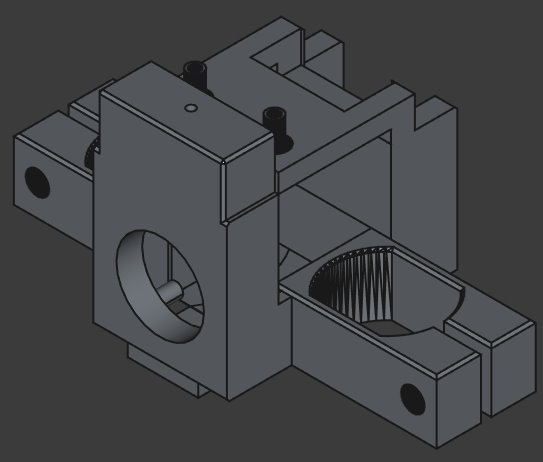
\includegraphics[width=\textwidth]{images/cad_gunarm_v2_front.jpg}
        \caption{Geschützarm Version 2 - Frontansicht}
    \end{subfigure}
    \hfill
    \begin{subfigure}[b]{0.45\textwidth}
        \centering
        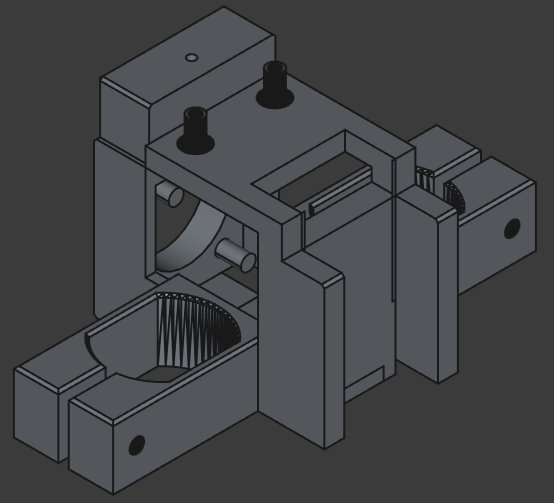
\includegraphics[width=\textwidth]{images/cad_gunarm_v2_back.jpg}
        \caption{Geschützarm Version 2 - Rückansicht}
    \end{subfigure}

    \caption{Geschützarm Version 2}
    \label{fig:gunarm_v2}
\end{figure}

Im Gegensatz zur Version 1 wird der Ultraschallsensor nun seitlich eingeführt anstatt von unten, siehe~\ref{fig:gunarm_v2}. Problematisch waren dabei die beschränkten Platzverhältnisse, da die Schrittmotoren näher am Kanonenrohr angebracht wurden als im vorherigen Entwurf. Außerdem wurden die zuvor angedachten Montagepunkte am Magazin wieder entfernt. Die Zusammenführung des Geschützarms mit dem Magazin erfolgte deshalb mittels Modellbaukleber.

\section{Montagehalterung Motortreiber (Specht)}

Für die ersten Funktionstests wurden die Pololu-Motoren provisorisch auf Kork-Schnipseln montiert. Dieses Vorgehen ermöglichte eine zügige Inbetriebnahme, jedoch erwies es sich hinsichtlich Stabilität und Sicherheit als unzureichend. Im Rahmen der Tests kam es zum Abrutschen eines Motors von der Korkunterlage, was zu einer kurzfristigen Wärmeentwicklung und Geruchsbildung führte. Glücklicherweise wurde eine Beschädigung der Hardware vermieden.

\begin{figure}[h]
    \centering

    \begin{subfigure}[b]{0.25\textwidth}
        \centering
        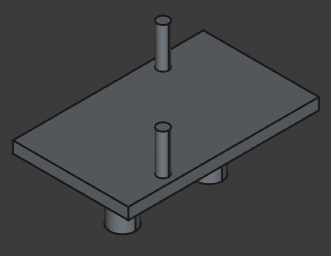
\includegraphics[width=\textwidth]{images/cad_polulu_front.png}
        \caption{Polulu - Draufsicht}
    \end{subfigure}
    \hspace{0.05\textwidth} % Adjust this value as needed
    \begin{subfigure}[b]{0.25\textwidth}
        \centering
        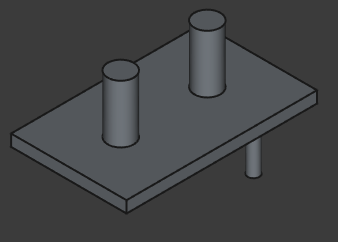
\includegraphics[width=\textwidth]{images/cad_polulu_back.png}
        \caption{Polulu - Bodensicht}
    \end{subfigure}

    \caption{Montagehalterung für Pololu-Motortreiber}
    \label{fig:pololu_mounting}
\end{figure}

Für die finale Abnahme wurde daher ein dauerhaftes und sicheres Montagesystem umgesetzt, das ein sauberes und zuverlässiges Setup gewährleistet. Wie in Abbildung~\ref{fig:pololu_mounting} zu sehen, kann die Halterung direkt auf der Montageplatte des Fahrzeugs geklippt werden.

\section{Dualshock4 Treiber (Becker)}

Gemäß der Anforderung ist die Steuerung des Fahrzeugs sowie der Geschützplattform durch einen DualShock4-Controller vorgesehen. 
Einerseits dient dies dem Testen der Plattformsteuerung für den späteren Betrieb der KI. 
Des Weiteren fungiert sie als Gamification-Element. 
Das Ziel ist die Steigerung des Nutzens und der Freude an dem Projekt, indem eine bekannte Steuerungsmethode verwendet wird, welche die Benutzerfreundlichkeit erhöht.

Für die Realisierung dieser Funktionalität wurde ein spezieller Treiber entwickelt, der den Zustand des Controllers in regelmäßigen Abständen an den ESP-32 übermittelt. 
Darüber hinaus umfasste mein Wunsch eine Funktion, die Vibrationen und Farbwechsel am Gamepad auslöst, und zwar vom Mikrocontroller aus.

\subsection{Übertragung}

Vor jeglicher Datenübertragung muss zunächst eine Kopplung per Bluetooth hergestellt werden. 
Der Sony Dualshock 4 Controller verwendet in diesem Fall den Bluetooth Classic 4.0 Standard.
Für die Verbindung des Controllers mit den Geräten ist im Flash-Speicher des Gamepads eine MAC-Adresse gespeichert. 
Beim Anschalten des Controllers wird versucht, Kontakt zu dieser Adresse aufzubauen.
Unter normalen Betriebsbedingungen wäre dies die Adresse der PlayStation4-Konsole. 
Für unser Projekt wurde jedoch die gespeicherte MAC-Adresse mit der des ESP-32 überschrieben.
Nach dem Einschalten unternimmt das Gamepad sofort den Versuch, sich mit dem Mikrocontroller zu verbinden.

Die Übertragung der Daten zwischen Gamepad und Mikrocontroller erfolgt mittels sogenannter HID-Reports.
HID-Reports sind binäre Datenstrukturen, welche die Reihenfolge der Informationen festlegen.
Die Struktur der Reports wurde von Sony nicht öffentlich zur Verfügung gestellt. 
Allerdings war es einigen Personen möglich, durch Reverse-Engineering wichtige Felder zu ermitteln \cite{esp_ds4_hid_reports}.

Das Human Interface Device (HID)-Protokoll ist ein standardisiertes Kommunikationsprotokoll zur Übertragung von Eingabe- und Steuerdaten zwischen Peripheriegeräten (z.B. Tastaturen, Mäusen, Gamepads) und einem Host-System. 
Es wurde ursprünglich für USB spezifiziert \cite{esp_usb_hid_spec} und später für Bluetooth Classic übernommen.

\begin{figure}[ht]
    \centering
    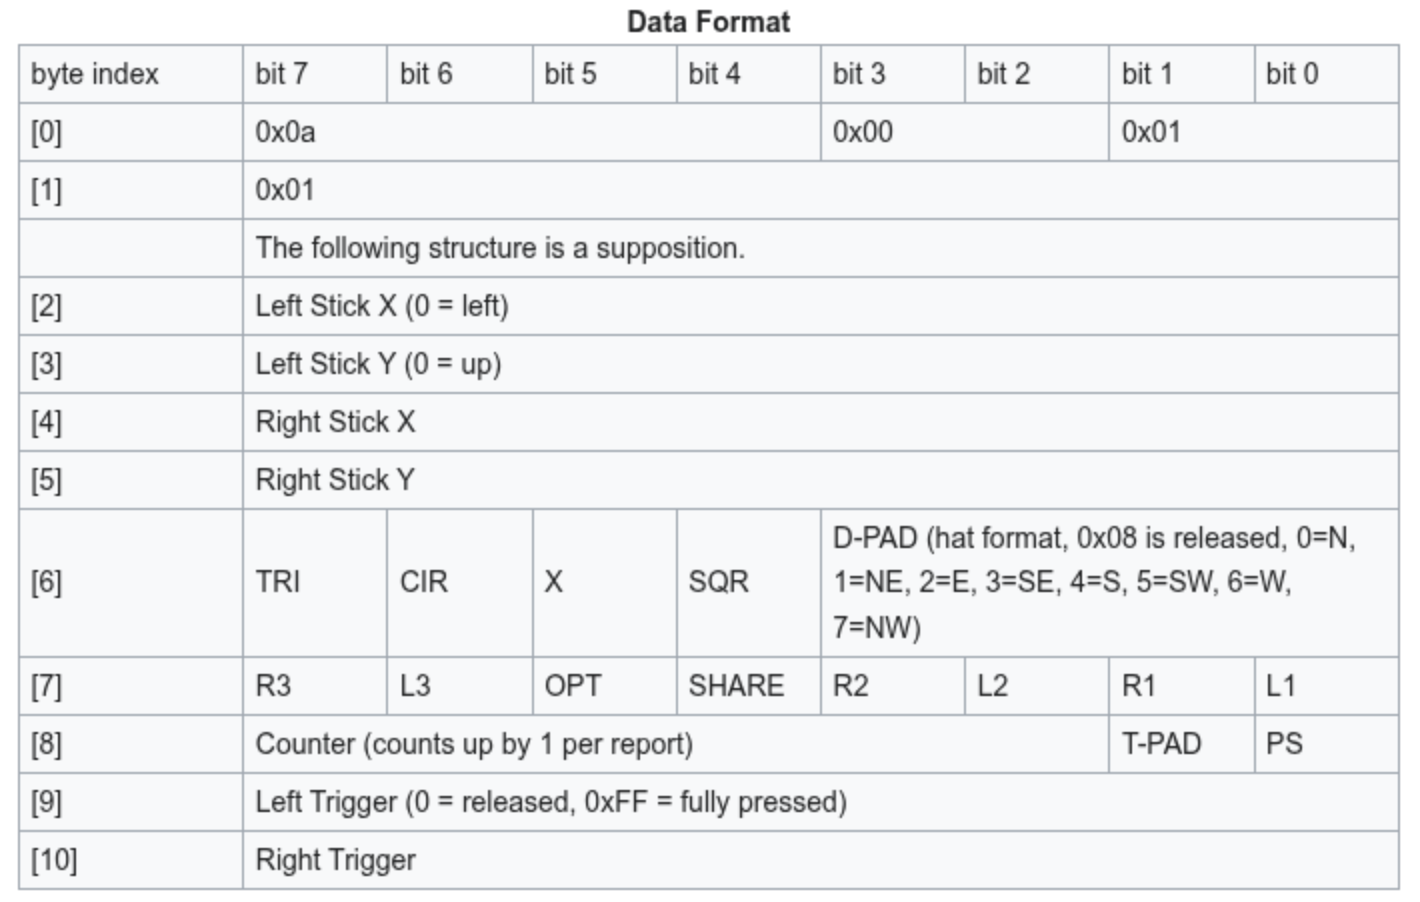
\includegraphics[width=0.7\textwidth]{images/becker_esp32_ds4_report.png}
    \caption{Beispielhafter Aufbau eines HID-Reports aus \cite{esp_ds4_hid_reports}}
\end{figure}

\subsection{Version 1: eigens entwickelter Treiber}

Eine Websuche nach existierenden DualShock-4-Treibern für das ESP-IDF brachte zunächst nur veraltete Implementierungen zutage, die auf nicht mehr unterstützten APIs basierten. 
Zahlreiche andere Ansätze zielten ausschließlich auf das Arduino-Framework ab und ließen sich daher nur eingeschränkt oder gar nicht in ein ESP-IDF-basiertes Projekt integrieren.

Da die Struktur der vom Gamepad gesendeten HID-Reports dank Reverse Engineering bekannt war und das ESP-IDF über eine Bluetooth-HID-Host-API verfügte \cite{esp_hib_bt_api}, wurde im ersten Ansatz ein eigener Treiber entwickelt.

Der Verbindungsaufbau verlief problemlos, und zu Beginn wurden die Input-Reports korrekt empfangen. 
Nach kurzer Zeit fror die Datenübertragung jedoch ein, obwohl alle anderen Tasks auf dem System weiterhin fehlerfrei ausgeführt wurden. 
Recherchen ergaben, dass dieses Verhalten auch von anderen Nutzern beobachtet wurde \cite{esp_hib_bt_api_issues}. 
Als Ursache wird die vergleichsweise hohe Sendefrequenz des Controllers vermutet, die laut Nutzertests bei über 700 Hz liegt \cite{esp_ds4_hid_reports}.

Um den Overhead in der Callback-Funktion für empfangene Reports zu reduzieren, wurde ein Zeitfilter implementiert. 
Ein Timer prüft beim Eintreffen eines Reports, ob seit dem letzten verarbeiteten Report mindestens $16.\overline{6}$ ms (entsprechend 60 Hz) vergangen sind. 
Ist dies der Fall, wird der aktuelle Report in eine durch FreeRTOS bereitgestellte Queue eingereiht. 
Diese wird von einem separaten Task abgearbeitet, der die Reports auf der Konsole protokolliert. 
Auf diese Weise konnte das Logging, das potenziell blockierend wirkt, vom zeitkritischen Pfad entkoppelt werden.

Obwohl diese Maßnahme die Zeitspanne, in der die Daten stabil übertragen wurden, verlängerte, wurde das zugrundeliegende Problem damit nicht vollständig gelöst. 
Nach einigen Minuten unterbrach der Controller die Übertragung der Reports erneut, obwohl die Status-LED weiterhin eine aktive Bluetooth-Verbindung anzeigte.

Da der ESP-32 in dieser Anwendung zusätzlich weitere zeitkritische Komponenten wie den Motortreiber verwalten muss, ist die Stabilität und Effizienz des Treibers von zentraler Bedeutung.
Aus diesem Grund wurde entschieden, die Entwicklung eines eigenen Treibers nicht weiter zu verfolgen und stattdessen nach einer robusteren und getesteten Alternative zu suchen.

\subsection{Version 2: Treiber basierend auf der Bluepad32 Bibliothek}

\subsection{Testing}

Um den funktionierenden Treiber zu testen wurden zwei Tasks auf dem ESP-32 erstellt:

\begin{itemize}
    \item \textbf{Input-Test Task}: Dieser Task wartet vor jedem Schleifendurchlauf auf verbinden, das bedeutet er ist so lange blockiert, bis der Dualshock-Controller die Verbindung hergestellt hat.
    Dann wartet er an der Input Queue bis der Controller einen Zustandsreport schickt. Dieser wir dann aus der Queue entnommen und auf der Konsole ausgegeben. Zuletzt wird $16.\overline{6}$ ms (60 Hz) gewartet.
    \item \textbf{Output-Test Task}: Hier wird ebenfalls blockiert bis das Gamepad verbunden ist. Nach dem die Verbindung aufgebaut ist wird je ein Vibrations- und Farbwechselevent in die Queue gelegt. 
    Da dass Vibrationsevent eine Dauer von 100 ms bekommen hat wird hier 100 ms gewartet.
\end{itemize}

Mit diesem simplen Testsetup konnten alle Funktionen des Controller getestet werden. 
Auch das Fortfahren nach einem Verbindungsabbruch konnten durch Aus- und Einschalten des Gamepads getestet werden. 

Bei Testen fiel weiterhin auf, dass die Batteriestandswarnung dauerhaft ausgelöst war, ein Blick auf die Input Werte zeigte, dass der Controller eine komplette leere Batterie anzeigte. 
Auch nach dem Aufladen fielen die Werte schnell wieder auf 0, obwohl am PC ganz andere Ladestände angezeigt wurden. (WIP!)

\section{Platformsteuerung (Becker)}

Die sogenannte Plattformsteuerung bezeichnet alle technischen Komponenten, die erforderlich sind, um die Plattform in ihrer Rotation, vertikalen Neigung sowie für die Abgabe eines Schusses zu steuern.

Für den genannten Zweck werden folgende Komponenten benötigt:

\begin{itemize}
    \item \textbf{Drehung und Neigung}
    \begin{itemize}
        \item zwei MG996R Servo Motoren
    \end{itemize}
    \item \textbf{Schussabgabe}
    \begin{itemize}
        \item zwei DC-Motoren (Flywheels)
        \item MG92B Servo Motor
    \end{itemize}
\end{itemize}

Da die maximale Ausgangsstärke eines GPIO-PINs des ESP-32 mit 40mA \cite[S.~53]{esp_datasheet} für die benötigten Motoren nicht ausreicht \cite{esp_platform_flywheel_motor,esp_platform_small_servo,esp_platform_servo}, wurden entsprechende Treiberbaords verwendet.
Konkret handelt es sich hierbei um ein PCA9685 PWM-Treiberboard für die Servomotoren und um per PWM steuerbare MOSFET-Module für die Flywheel-Motoren.

In der nachfolgenden Sektion wird der Entwurf des Codes erörtert, der erforderlich ist, um die genannten Teile anzusteuern.

\subsection{PWM Board Treiber (Becker)}

Das PCA9685 PWM-Treiberboard gestattet die gleichzeitige Anbindung von bis zu 16 Servomotoren.
Für die Stromversorgung steht ein Eingang mit einer Spannung von 5 Volt zur Verfügung.

Die Steuerung des Boards erfolgt durch das Schreiben verschiedener Werte in Konfigurationsregister, wobei das I²C-Protokoll zum Einsatz kommt. 
Der vorliegende Treiber wurde aus der Portierung eines bereits bestehenden Treibers \cite{esp_pca9685_blueprint} entwickelt, welcher in der Programmiersprache C++ implementiert war. 
Es wurde bewusst nur die Funktionalität portiert, die für den Umfang des Projekts von Relevanz war. 
Der Treiber umfasst demzufolge lediglich drei Funktionen:

\begin{itemize}
    \item \textbf{pca9685\_init}: Die Funktion erhält die gewünschte Konfiguration für das Board (beispielsweise die Bus-Adresse, die SDA- und SCL-Ports für den I²C-Bus) und initialisiert den I²C-Bus. 
    Im Anschluss registriert sie das Treiberboard und konfiguriert schließlich das Board mit der gewünschten PWM-Frequenz.
    \item \textbf{pca9685\_set\_pwm\_on\_off}: Mithilfe dieser Funktion besteht nun die Möglichkeit, einen Motor auf einem der 16 Kanäle zu steuern. 
    Der Parameter \textit{ON} ist eine 12-Bit Zahl beschreibt hierbei den Zeitpunkt in der Phase, an welchem der Ausgang auf 5 Volt geschalten wird. 
    \textit{OFF}, ebenfalls eine 12-Bit Zahl bezeichnet den Zeitpunkt, zu welchem der Ausgang wieder auf 0 Volt geregelt wird. 
    Eine grafische Veranschaulichung ist in Abbildung \ref{fig:esp_pca9685_on_off} ersichtlich. 
    Da für die Ansteuerung der Servo Motoren keine symmetrischen PWM-Signale benötigt werden, wird der Parameter \textit{ON} im Folgenden immer den Wert 0 annehmen.

    \begin{figure}[ht]
        \centering
        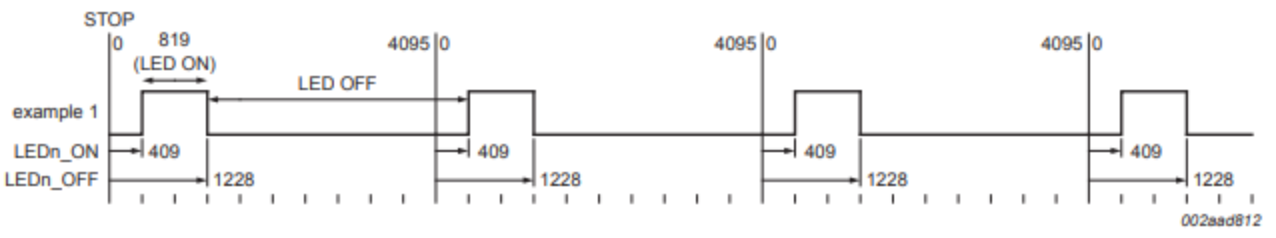
\includegraphics[width=\textwidth]{images/becker_esp_pca9685.png}
        \caption{Erklärung ON\slash OFF Parameter für PCA9685 aus \cite[S.~17]{esp_pca9685_datasheet}}
        \label{fig:esp_pca9685_on_off}
    \end{figure}

    \item \textbf{pca9685\_set\_off}: Mittels dieser Funktion kann das PWM-Signal auf einem bestimmten Kanal deaktiviert werden.
\end{itemize}

Auf Basis dieses Treiber wurden im nächsten Schritt zwei Interfaces programmiert: 
Einerseits das Interface zur Plattform-Kontrolle und andererseits das Interface zur Schusskontrolle, welches zusätzlich der Logik zur Ansteuerung der Flywheel-Motoren enthält.

\subsection{Ansteuerung der Servo-Motoren (Becker)}

Um nun die Plattform sowohl manuell über den DualShock4-Controller als auch semi-automatisch per künstlicher Intelligenz über MQTT präzise steuern zu können, wurde ein Interface entwickelt, das die Ansteuerung eines Motors an eine bestimmte Position erlaubt. 

In diesem Kontext wird mit der Einheit Grad gearbeitet. 
Ein Blick in die Referenz \cite{esp_servo_control} der Servo-Motoren zeigt, dass durch die Einstellung der Duty-Cycle-Länge des PWM-Signals eine Drehung auf eine bestimmte Grad-Position erreicht wird. 
Im ersten Schritt wurden die \textit{OFF} Werte für die Punkte \ang{-90} (max. Drehung nach links), \ang{0} und \ang{90} (max. Drehung nach rechts) manuell ermittelt.
Die absoluten Werte für die Drehungen werden im Folgenden als $value_{-90^\circ}$, $value_{0^\circ}$ und $value_{90^\circ}$ bezeichnet.

Für die Berechnung des Zielwerts $value_{off}$ für den \textit{OFF} Wert des PWM-Board-Treibers aus einem gegebenen Winkel wird Formel \ref{eq:pwm_to_duty} verwendet.

\begin{gather}
    \begin{aligned}
    &\text{Sei } \theta \text{ der gewünschte Winkel,} \\
    &|\theta| = \text{Betrag von } \theta \\
    &n_3 = \left\lfloor \frac{|\theta|}{3} \right\rfloor \\
    &n_2 = |\theta| - n_3 \\
    &s = 2 \cdot n_2 + 3 \cdot n_3 \\
    &\tilde{s} =
    \begin{cases}
    s, & \theta > 0 \\
    -s, & \theta \leq 0
    \end{cases} \\
    &value_{off} = value_{zero} + \tilde{s}
    \end{aligned}
    \label{eq:pwm_to_duty}
\end{gather}

Die Idee der Formel beruht auf der Tatsache, dass die Differenz aus $value_{90^\circ}$ bzw. $value_{-90^\circ}$ und $value_{0^\circ}$ gebildet und anschließend gleichmäßig auf den Bereich von $]1, 90[$, also auf 90 Werte, aufgeteilt wird. 

Für jedes zusätzliche Grad Rotation um den Nullpunkt müssten demnach entweder $2.\overline{3}$ addiert oder subtrahiert werden.
Da dies in Anbetracht der Verwendung von Festkommazahlen nicht realisierbar wäre, erscheint die naheliegende Idee, den Wert zu runden. 
Diese Praktik würde jedoch im Zeitverlauf zu einer zunehmenden Abweichung und folglich zu einem Verlust an Präzision führen.
Um das genannte Problem zu vermeiden, wird der \textit{OFF} Wert für jedes dritte Grad Drehung um den Faktor 3 verändert und für jedes andere Grad um Faktor 2.
Die Formel \ref{eq:pwm_to_duty} berechnet dabei in $n_3$ die Anzahl der Faktor-3-Drehungen und in $n_2$ die Anzahl der Faktor-2-Drehungen.
Ausgehend davon wird $value_{0^\circ}$ verändert.

Das Endergebnis stellt eine Funktion dar, mittels derer eine präzise gradweise Ansteuerung beider Plattformachsen möglich ist.

Darüber hinaus wurde im Interface ein Clipping der Werte als Sicherheitmechanismus integriert. Im Zuge der Initialisierung des Plattforminterfaces muss für jede Achse ein Startwinkel sowie ein linker und rechter Stopwinkel angegeben werden.
Sollte es bei der Steuerung durch den Dualshock4-Controller in dessen Regelschleife oder in der KI-Berechnung zu einem fehlerhaften Gradwert kommen, wird dieser Wert automatisch an den nächstgelegenen Stopwinkel geclippt. 
Durch diese Maßnahme werden potenzielle Materialschäden, die durch fehlerhafte Drehungen verursacht werden könnten, verhindert.

Die Realisierung der Ansteuerung des kleinen Servos, dessen Funktion darin besteht, die Nerf-Darts in die Flywheel-Motoren zu schieben, würde durch die Verwendung dieser Art der Ansteuerung zu einer unnötigen Komplexität führen.
Daher wurde für diesen Motor lediglich eine Startposition (Geschütztrigger ganz hinten; Dart kann in das Magazin fallen) und eine Endposition (Geschütztrigger ganz vorne; Dart wurde in die Flywheels geschoben) durch manuelles Einsetzen von \textit{OFF} Werten festgelegt.
Wird nun ein Schuss ausgelöst, so fährt der Servo-Motor zunächst in seine Endposition und von dort aus wieder zurück in seine Startposition.

\subsection{Ansteuerung der Flywheel Motoren (Becker, Koch, Wohlrab)}

Für die Vervollständigung des Fire-Control Interfaces wird nun noch die Ansteuerung der Flywheel-Motoren benötigt.
In dem vorliegenden Projekt erfolgt die Steuerung der beiden Gleichstrommotoren jeweils durch ein Power-MOSFET-Modul.

Die Funktionsweise des Modul lässt sich folgendermaßen beschreiben:

\begin{itemize}
    \item Auf einer Seite wird der Eingangstrom, in unserem Fall 5V, vom Stromverteiler eingeführt.
    \item Andererseits wird der Ausgang jeweils mit einem Motor verbunden.
    \item Die am Ausgang ausgegebene Spannung kann über einen PWM-Pin geregelt werden \cite{esp_platform_flywheel_motor}.
\end{itemize}

Die Wahl fiel auf dieses relativ simple Modul, da lediglich die Anforderung bestand, dass sich die Motoren bei der Schussabgabe möglichst schnell drehen sollen.
Im Rahmen dieses Projekts waren keine Änderungen der Richtung oder präzisere Steuerung erforderlich.

Im Rahmen des manuellen Tests wurde festgestellt, dass zur Erzielung eines optimalen Schussbildes eine Versorgung der Motoren mit 5 Volt erforderlich ist. 
Infolgedessen beträgt der Duty-Cycle entweder 0 oder 100 Prozent.
Daher wurde der ursprüngliche PWM-Code letztlich auf das reine Ein- und Ausschalten eines GPIO-Pins reduziert.

\section{Integration (Becker, Specht)}
\section{Dualshock4 Treiber (Becker)}

Gemäß der Anforderung ist die Steuerung des Fahrzeugs sowie der Geschützplattform durch einen DualShock4-Controller vorgesehen. 
Einerseits dient dies dem Testen der Plattformsteuerung für den späteren Betrieb der KI. 
Des Weiteren fungiert sie als Gamification-Element. 
Das Ziel ist die Steigerung des Nutzens und der Freude an dem Projekt, indem eine bekannte Steuerungsmethode verwendet wird, welche die Benutzerfreundlichkeit erhöht.

Für die Realisierung dieser Funktionalität wurde ein spezieller Treiber entwickelt, der den Zustand des Controllers in regelmäßigen Abständen an den ESP-32 übermittelt. 
Darüber hinaus umfasste mein Wunsch eine Funktion, die Vibrationen und Farbwechsel am Gamepad auslöst, und zwar vom Mikrocontroller aus.

\subsection{Übertragung}

Vor jeglicher Datenübertragung muss zunächst eine Kopplung per Bluetooth hergestellt werden. 
Der Sony Dualshock 4 Controller verwendet in diesem Fall den Bluetooth Classic 4.0 Standard.
Für die Verbindung des Controllers mit den Geräten ist im Flash-Speicher des Gamepads eine MAC-Adresse gespeichert. 
Beim Anschalten des Controllers wird versucht, Kontakt zu dieser Adresse aufzubauen.
Unter normalen Betriebsbedingungen wäre dies die Adresse der PlayStation4-Konsole. 
Für unser Projekt wurde jedoch die gespeicherte MAC-Adresse mit der des ESP-32 überschrieben.
Nach dem Einschalten unternimmt das Gamepad sofort den Versuch, sich mit dem Mikrocontroller zu verbinden.

Die Übertragung der Daten zwischen Gamepad und Mikrocontroller erfolgt mittels sogenannter HID-Reports.
HID-Reports sind binäre Datenstrukturen, welche die Reihenfolge der Informationen festlegen.
Die Struktur der Reports wurde von Sony nicht öffentlich zur Verfügung gestellt. 
Allerdings war es einigen Personen möglich, durch Reverse-Engineering wichtige Felder zu ermitteln \cite{esp_ds4_hid_reports}.

Das Human Interface Device (HID)-Protokoll ist ein standardisiertes Kommunikationsprotokoll zur Übertragung von Eingabe- und Steuerdaten zwischen Peripheriegeräten (z.B. Tastaturen, Mäusen, Gamepads) und einem Host-System. 
Es wurde ursprünglich für USB spezifiziert \cite{esp_usb_hid_spec} und später für Bluetooth Classic übernommen.

\begin{figure}[ht]
    \centering
    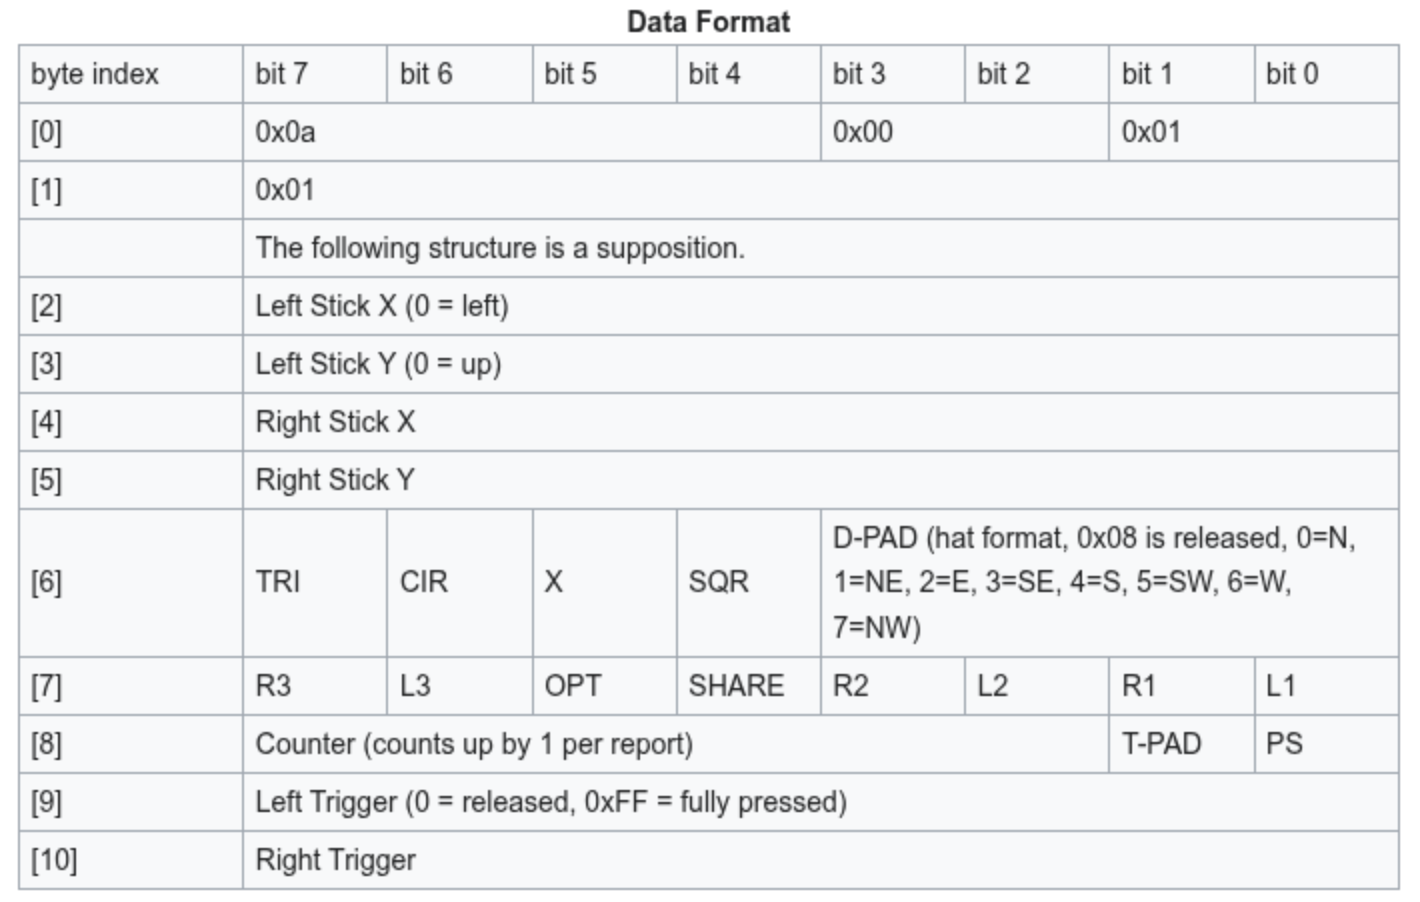
\includegraphics[width=0.7\textwidth]{images/becker_esp32_ds4_report.png}
    \caption{Beispielhafter Aufbau eines HID-Reports aus \cite{esp_ds4_hid_reports}}
\end{figure}

\subsection{Version 1: eigens entwickelter Treiber}

Eine Websuche nach existierenden DualShock-4-Treibern für das ESP-IDF brachte zunächst nur veraltete Implementierungen zutage, die auf nicht mehr unterstützten APIs basierten. 
Zahlreiche andere Ansätze zielten ausschließlich auf das Arduino-Framework ab und ließen sich daher nur eingeschränkt oder gar nicht in ein ESP-IDF-basiertes Projekt integrieren.

Da die Struktur der vom Gamepad gesendeten HID-Reports dank Reverse Engineering bekannt war und das ESP-IDF über eine Bluetooth-HID-Host-API verfügte \cite{esp_hib_bt_api}, wurde im ersten Ansatz ein eigener Treiber entwickelt.

Der Verbindungsaufbau verlief problemlos, und zu Beginn wurden die Input-Reports korrekt empfangen. 
Nach kurzer Zeit fror die Datenübertragung jedoch ein, obwohl alle anderen Tasks auf dem System weiterhin fehlerfrei ausgeführt wurden. 
Recherchen ergaben, dass dieses Verhalten auch von anderen Nutzern beobachtet wurde \cite{esp_hib_bt_api_issues}. 
Als Ursache wird die vergleichsweise hohe Sendefrequenz des Controllers vermutet, die laut Nutzertests bei über 700 Hz liegt \cite{esp_ds4_hid_reports}.

Um den Overhead in der Callback-Funktion für empfangene Reports zu reduzieren, wurde ein Zeitfilter implementiert. 
Ein Timer prüft beim Eintreffen eines Reports, ob seit dem letzten verarbeiteten Report mindestens $16.\overline{6}$ ms (entsprechend 60 Hz) vergangen sind. 
Ist dies der Fall, wird der aktuelle Report in eine durch FreeRTOS bereitgestellte Queue eingereiht. 
Diese wird von einem separaten Task abgearbeitet, der die Reports auf der Konsole protokolliert. 
Auf diese Weise konnte das Logging, das potenziell blockierend wirkt, vom zeitkritischen Pfad entkoppelt werden.

Obwohl diese Maßnahme die Zeitspanne, in der die Daten stabil übertragen wurden, verlängerte, wurde das zugrundeliegende Problem damit nicht vollständig gelöst. 
Nach einigen Minuten unterbrach der Controller die Übertragung der Reports erneut, obwohl die Status-LED weiterhin eine aktive Bluetooth-Verbindung anzeigte.

Da der ESP-32 in dieser Anwendung zusätzlich weitere zeitkritische Komponenten wie den Motortreiber verwalten muss, ist die Stabilität und Effizienz des Treibers von zentraler Bedeutung.
Aus diesem Grund wurde entschieden, die Entwicklung eines eigenen Treibers nicht weiter zu verfolgen und stattdessen nach einer robusteren und getesteten Alternative zu suchen.

\subsection{Version 2: Treiber basierend auf der Bluepad32 Bibliothek}

\subsection{Testing}

Um den funktionierenden Treiber zu testen wurden zwei Tasks auf dem ESP-32 erstellt:

\begin{itemize}
    \item \textbf{Input-Test Task}: Dieser Task wartet vor jedem Schleifendurchlauf auf verbinden, das bedeutet er ist so lange blockiert, bis der Dualshock-Controller die Verbindung hergestellt hat.
    Dann wartet er an der Input Queue bis der Controller einen Zustandsreport schickt. Dieser wir dann aus der Queue entnommen und auf der Konsole ausgegeben. Zuletzt wird $16.\overline{6}$ ms (60 Hz) gewartet.
    \item \textbf{Output-Test Task}: Hier wird ebenfalls blockiert bis das Gamepad verbunden ist. Nach dem die Verbindung aufgebaut ist wird je ein Vibrations- und Farbwechselevent in die Queue gelegt. 
    Da dass Vibrationsevent eine Dauer von 100 ms bekommen hat wird hier 100 ms gewartet.
\end{itemize}

Mit diesem simplen Testsetup konnten alle Funktionen des Controller getestet werden. 
Auch das Fortfahren nach einem Verbindungsabbruch konnten durch Aus- und Einschalten des Gamepads getestet werden. 

Bei Testen fiel weiterhin auf, dass die Batteriestandswarnung dauerhaft ausgelöst war, ein Blick auf die Input Werte zeigte, dass der Controller eine komplette leere Batterie anzeigte. 
Auch nach dem Aufladen fielen die Werte schnell wieder auf 0, obwohl am PC ganz andere Ladestände angezeigt wurden. (WIP!)

\section{Platformsteuerung (Becker)}

Die sogenannte Plattformsteuerung bezeichnet alle technischen Komponenten, die erforderlich sind, um die Plattform in ihrer Rotation, vertikalen Neigung sowie für die Abgabe eines Schusses zu steuern.

Für den genannten Zweck werden folgende Komponenten benötigt:

\begin{itemize}
    \item \textbf{Drehung und Neigung}
    \begin{itemize}
        \item zwei MG996R Servo Motoren
    \end{itemize}
    \item \textbf{Schussabgabe}
    \begin{itemize}
        \item zwei DC-Motoren (Flywheels)
        \item MG92B Servo Motor
    \end{itemize}
\end{itemize}

Da die maximale Ausgangsstärke eines GPIO-PINs des ESP-32 mit 40mA \cite[S.~53]{esp_datasheet} für die benötigten Motoren nicht ausreicht \cite{esp_platform_flywheel_motor,esp_platform_small_servo,esp_platform_servo}, wurden entsprechende Treiberbaords verwendet.
Konkret handelt es sich hierbei um ein PCA9685 PWM-Treiberboard für die Servomotoren und um per PWM steuerbare MOSFET-Module für die Flywheel-Motoren.

In der nachfolgenden Sektion wird der Entwurf des Codes erörtert, der erforderlich ist, um die genannten Teile anzusteuern.

\subsection{PWM Board Treiber (Becker)}

Das PCA9685 PWM-Treiberboard gestattet die gleichzeitige Anbindung von bis zu 16 Servomotoren.
Für die Stromversorgung steht ein Eingang mit einer Spannung von 5 Volt zur Verfügung.

Die Steuerung des Boards erfolgt durch das Schreiben verschiedener Werte in Konfigurationsregister, wobei das I²C-Protokoll zum Einsatz kommt. 
Der vorliegende Treiber wurde aus der Portierung eines bereits bestehenden Treibers \cite{esp_pca9685_blueprint} entwickelt, welcher in der Programmiersprache C++ implementiert war. 
Es wurde bewusst nur die Funktionalität portiert, die für den Umfang des Projekts von Relevanz war. 
Der Treiber umfasst demzufolge lediglich drei Funktionen:

\begin{itemize}
    \item \textbf{pca9685\_init}: Die Funktion erhält die gewünschte Konfiguration für das Board (beispielsweise die Bus-Adresse, die SDA- und SCL-Ports für den I²C-Bus) und initialisiert den I²C-Bus. 
    Im Anschluss registriert sie das Treiberboard und konfiguriert schließlich das Board mit der gewünschten PWM-Frequenz.
    \item \textbf{pca9685\_set\_pwm\_on\_off}: Mithilfe dieser Funktion besteht nun die Möglichkeit, einen Motor auf einem der 16 Kanäle zu steuern. 
    Der Parameter \textit{ON} ist eine 12-Bit Zahl beschreibt hierbei den Zeitpunkt in der Phase, an welchem der Ausgang auf 5 Volt geschalten wird. 
    \textit{OFF}, ebenfalls eine 12-Bit Zahl bezeichnet den Zeitpunkt, zu welchem der Ausgang wieder auf 0 Volt geregelt wird. 
    Eine grafische Veranschaulichung ist in Abbildung \ref{fig:esp_pca9685_on_off} ersichtlich. 
    Da für die Ansteuerung der Servo Motoren keine symmetrischen PWM-Signale benötigt werden, wird der Parameter \textit{ON} im Folgenden immer den Wert 0 annehmen.

    \begin{figure}[ht]
        \centering
        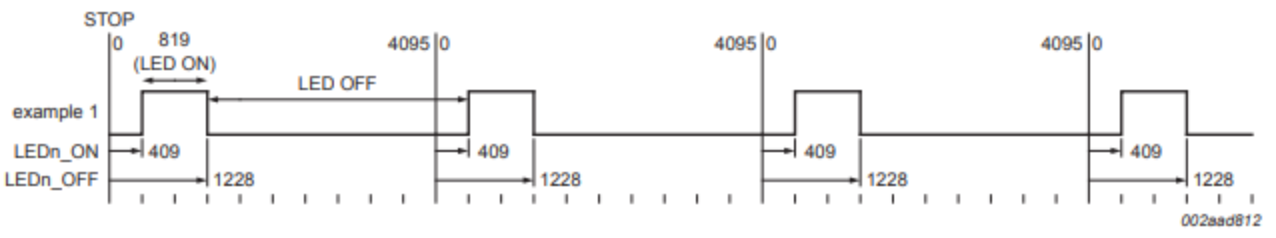
\includegraphics[width=\textwidth]{images/becker_esp_pca9685.png}
        \caption{Erklärung ON\slash OFF Parameter für PCA9685 aus \cite[S.~17]{esp_pca9685_datasheet}}
        \label{fig:esp_pca9685_on_off}
    \end{figure}

    \item \textbf{pca9685\_set\_off}: Mittels dieser Funktion kann das PWM-Signal auf einem bestimmten Kanal deaktiviert werden.
\end{itemize}

Auf Basis dieses Treiber wurden im nächsten Schritt zwei Interfaces programmiert: 
Einerseits das Interface zur Plattform-Kontrolle und andererseits das Interface zur Schusskontrolle, welches zusätzlich der Logik zur Ansteuerung der Flywheel-Motoren enthält.

\subsection{Ansteuerung der Servo-Motoren (Becker)}

Um nun die Plattform sowohl manuell über den DualShock4-Controller als auch semi-automatisch per künstlicher Intelligenz über MQTT präzise steuern zu können, wurde ein Interface entwickelt, das die Ansteuerung eines Motors an eine bestimmte Position erlaubt. 

In diesem Kontext wird mit der Einheit Grad gearbeitet. 
Ein Blick in die Referenz \cite{esp_servo_control} der Servo-Motoren zeigt, dass durch die Einstellung der Duty-Cycle-Länge des PWM-Signals eine Drehung auf eine bestimmte Grad-Position erreicht wird. 
Im ersten Schritt wurden die \textit{OFF} Werte für die Punkte \ang{-90} (max. Drehung nach links), \ang{0} und \ang{90} (max. Drehung nach rechts) manuell ermittelt.
Die absoluten Werte für die Drehungen werden im Folgenden als $value_{-90^\circ}$, $value_{0^\circ}$ und $value_{90^\circ}$ bezeichnet.

Für die Berechnung des Zielwerts $value_{off}$ für den \textit{OFF} Wert des PWM-Board-Treibers aus einem gegebenen Winkel wird Formel \ref{eq:pwm_to_duty} verwendet.

\begin{gather}
    \begin{aligned}
    &\text{Sei } \theta \text{ der gewünschte Winkel,} \\
    &|\theta| = \text{Betrag von } \theta \\
    &n_3 = \left\lfloor \frac{|\theta|}{3} \right\rfloor \\
    &n_2 = |\theta| - n_3 \\
    &s = 2 \cdot n_2 + 3 \cdot n_3 \\
    &\tilde{s} =
    \begin{cases}
    s, & \theta > 0 \\
    -s, & \theta \leq 0
    \end{cases} \\
    &value_{off} = value_{zero} + \tilde{s}
    \end{aligned}
    \label{eq:pwm_to_duty}
\end{gather}

Die Idee der Formel beruht auf der Tatsache, dass die Differenz aus $value_{90^\circ}$ bzw. $value_{-90^\circ}$ und $value_{0^\circ}$ gebildet und anschließend gleichmäßig auf den Bereich von $]1, 90[$, also auf 90 Werte, aufgeteilt wird. 

Für jedes zusätzliche Grad Rotation um den Nullpunkt müssten demnach entweder $2.\overline{3}$ addiert oder subtrahiert werden.
Da dies in Anbetracht der Verwendung von Festkommazahlen nicht realisierbar wäre, erscheint die naheliegende Idee, den Wert zu runden. 
Diese Praktik würde jedoch im Zeitverlauf zu einer zunehmenden Abweichung und folglich zu einem Verlust an Präzision führen.
Um das genannte Problem zu vermeiden, wird der \textit{OFF} Wert für jedes dritte Grad Drehung um den Faktor 3 verändert und für jedes andere Grad um Faktor 2.
Die Formel \ref{eq:pwm_to_duty} berechnet dabei in $n_3$ die Anzahl der Faktor-3-Drehungen und in $n_2$ die Anzahl der Faktor-2-Drehungen.
Ausgehend davon wird $value_{0^\circ}$ verändert.

Das Endergebnis stellt eine Funktion dar, mittels derer eine präzise gradweise Ansteuerung beider Plattformachsen möglich ist.

Darüber hinaus wurde im Interface ein Clipping der Werte als Sicherheitmechanismus integriert. Im Zuge der Initialisierung des Plattforminterfaces muss für jede Achse ein Startwinkel sowie ein linker und rechter Stopwinkel angegeben werden.
Sollte es bei der Steuerung durch den Dualshock4-Controller in dessen Regelschleife oder in der KI-Berechnung zu einem fehlerhaften Gradwert kommen, wird dieser Wert automatisch an den nächstgelegenen Stopwinkel geclippt. 
Durch diese Maßnahme werden potenzielle Materialschäden, die durch fehlerhafte Drehungen verursacht werden könnten, verhindert.

Die Realisierung der Ansteuerung des kleinen Servos, dessen Funktion darin besteht, die Nerf-Darts in die Flywheel-Motoren zu schieben, würde durch die Verwendung dieser Art der Ansteuerung zu einer unnötigen Komplexität führen.
Daher wurde für diesen Motor lediglich eine Startposition (Geschütztrigger ganz hinten; Dart kann in das Magazin fallen) und eine Endposition (Geschütztrigger ganz vorne; Dart wurde in die Flywheels geschoben) durch manuelles Einsetzen von \textit{OFF} Werten festgelegt.
Wird nun ein Schuss ausgelöst, so fährt der Servo-Motor zunächst in seine Endposition und von dort aus wieder zurück in seine Startposition.

\subsection{Ansteuerung der Flywheel Motoren (Becker, Koch, Wohlrab)}

Für die Vervollständigung des Fire-Control Interfaces wird nun noch die Ansteuerung der Flywheel-Motoren benötigt.
In dem vorliegenden Projekt erfolgt die Steuerung der beiden Gleichstrommotoren jeweils durch ein Power-MOSFET-Modul.

Die Funktionsweise des Modul lässt sich folgendermaßen beschreiben:

\begin{itemize}
    \item Auf einer Seite wird der Eingangstrom, in unserem Fall 5V, vom Stromverteiler eingeführt.
    \item Andererseits wird der Ausgang jeweils mit einem Motor verbunden.
    \item Die am Ausgang ausgegebene Spannung kann über einen PWM-Pin geregelt werden \cite{esp_platform_flywheel_motor}.
\end{itemize}

Die Wahl fiel auf dieses relativ simple Modul, da lediglich die Anforderung bestand, dass sich die Motoren bei der Schussabgabe möglichst schnell drehen sollen.
Im Rahmen dieses Projekts waren keine Änderungen der Richtung oder präzisere Steuerung erforderlich.

Im Rahmen des manuellen Tests wurde festgestellt, dass zur Erzielung eines optimalen Schussbildes eine Versorgung der Motoren mit 5 Volt erforderlich ist. 
Infolgedessen beträgt der Duty-Cycle entweder 0 oder 100 Prozent.
Daher wurde der ursprüngliche PWM-Code letztlich auf das reine Ein- und Ausschalten eines GPIO-Pins reduziert.

\section{Integration (Becker, Specht)}

\section{Gyrosensor Programmierung (Koch)}
Zu Beginn des Projekts war geplant den Gyrosensor MPU6050 zu nutzen, um die Position der Geschützplattform zu bestimmen, da eine kontinuierliche Bewegung um die eigene Achse aufgrund der Kabel nicht möglich ist. Dabei sollte der Sensor über den I2C-Bus mit dem Raspberry Pi 5 verbunden werden, um die Daten auszulesen und zu verarbeiten.
Der MPU6050 ist dabei ein 3-Achsen-Gyroskop und 3-Achsen-Beschleunigungssensor, welcher entsprechende Drehbewegungen und Beschleunigungen entlang der Raumachsen messen kann, welche für eine genaue Winkelbestimmung notwendig sind.

Nach kurzem Einlesen in die Dokumentation waren erste Rohdaten leicht auszulesen. Diese Rohdaten liegen in Form von 16 Bit in zwei Registern bereit und haben die Einheit $\mathit{LSB/g}$ für die Beschleunigungswerte und $\mathit{LSB/^\circ s}$ für die Gyroskop-Werte. Dies gilt es in tatsächliche physikalische Größen umzuwandeln, was bei unserem Projekt letztlich einem Winkel entspricht. 
Um die Beschleunigungswerte nutzen zu können, muss dafür mittels des Skalierungsfaktors die Fallbeschleunigung $\mathit{g}$ errechnet werden, indem man den erhaltenen Wert $x/16384$ rechnet. Die $16384$ ergeben sich aus der Dokumentation und entsprechen den LSB bei einem Messbereich von $\pm2g$, welches der Standardauflösung entspricht und auch die höchste Auflösung des MPU6050 für ist.
Ähnlich wird nun auch Winkelgeschwindigkeit ($\mathit{^\circ s}$) errechnet. Hierbei beträgt der Teiler standardmäßig $131$. \cite[S. 12-13]{raspberry_invensense_mpu6050_datasheet} 

Nach der Umrechnung der Rohdaten in physikalische Größen können nun die Neigungswinkel (Roll- und Pitch-Winkel) des Sensors berechnet werden. Diese ergeben sich aus der Richtung der Erdbeschleunigung relativ zum Sensor. 

Dazu wird die Erweiterung des Arkustangens genutzt, genauer gesagt die Funktion \texttt{atan2}, da sie im Gegensatz zum gewöhnlichen Arctangens auch die Orientierung in allen vier Quadranten berücksichtigt und somit stabile Winkelwerte über den gesamten Bereich von $-180^\circ$ bis $+180^\circ$ liefert. \cite{raspberry_matlab_atan2}

Die Winkelberechnung erfolgt nach der Formel \ref{eq:norms_to_angle}:

\begin{gather}
    \begin{aligned}
    \varphi_\text{pitch} &= \arctan2\left(a_y,\sqrt{a_x^2 + a_z^2}\right) \cdot \frac{180^\circ}{\pi} \\
    \varphi_\text{roll}  &= \arctan2\left(a_x,\sqrt{a_y^2 + a_z^2}\right) \cdot \frac{180^\circ}{\pi}
    \end{aligned}
    \label{eq:norms_to_angle}
\end{gather}


Hierbei sind $a_x$, $a_y$ und $a_z$ die normierten Beschleunigungswerte in $\mathit{g}$ (berechnet aus den Rohwerten durch Division durch $16384$). 

Die $atan2$-Funktion liefert den Winkel zwischen der positiven $x$-Achse und dem Punkt $(x, y)$ in der Ebene, wodurch Sprünge oder Mehrdeutigkeiten bei $90^\circ$ vermieden werden. \cite{raspberry_matlab_atan2}

Nachdem der Term im Code implementiert wurde, konnte ein starkes Rauschen beobachtet werden, was zunächst auf natürliche Schwankungen des Sensors zurückgeführt wurde, weshalb sich dazu entschieden wurde zuerst einen Komplementärfilter zu implementieren,
welcher allerdings das Problem nur bedingt beheben konnte. Deshalb wurde auch noch der Kalman-Filter ausgetestet, wodurch auch eine starke  Rauschunterdrückung festgestellt werden konnte, doch auch hier zeichnete sich ein überdurchschnittliches Rauschverhalten ab, weshalb der Fehler nicht mehr auf ein natürliches Rauschen zurückzuführen war.
Daraufhin wurde auch ein zweiter MPU6050 getestet, welcher ebenfalls dieses Verhalten aufwies, wodurch klar wurde, dass es sich hierbei um einen Programmierfehler handeln muss. Dieser konnte nach einiger Zeit auch herausgefunden werden und lag an der Interpretation der Rohdaten, 
welche fälschlicherweise als \texttt{int16\_t} statt \texttt{uint16\_t} interpretiert wurden.

Aufgrund der aufgewendeten Zeit für die Implementierung des Kalman-Filters sollte dieser aber trotzdem Anwendung im Projekt finden und wird in \ref{sec:kalman_filter} behandelt.

Wie Eingangs erwähnt, sollte der Gyrosensor MPU6050 genutzt werden, um die Position der Geschützplattform zu bestimmen, wofür der Winkel der Drehung um die eigene Achse benötigt wird. Dabei stellte sich heraus das der MPU6050 für diesen Wert zu einem starken Drift neigt, weshalb empfohlen wird diesen mit einem Magnetometer zu kombinieren \cite[S. 26]{raspberry_invensense_mpu6050_datasheet}.
Zur gleichen Zeit stellte sich heraus, dass diese Funktionalität nicht benötigt wird, da über die Servo-Motoren bereits ein Nullpunkt definiert werden konnte, weshalb der Gyrosensor letztlich nur noch für die Neigung der Geschützplattform genutzt wird, um diese als Debug-Information auf dem Webserver \ref{sec:Webserver} anzuzeigen.

\subsection{Kalman Filter Implementierung (Koch)}
\label{sec:kalman_filter}
Der Kalman-Filter ist ein Algorithmus zur Schätzung des Zustands eines dynamischen Systems. Er nutzt Messwerte mit einem mathematischen Modell, um aus verrauschten Daten optimale Schätzungen zu erzeugen und zu filtern, was insbesondere bei Sensoren mit Rauschen, wie dem MPU6050, von Bedeutung ist \cite{raspberry_rwth_kalman_2025}.
Die Berechnung des Kalman-Filters erfolgt nun mittels der Werte des Gyroskops, einer Zeitdifferenz und der zuvor berechneten Roll-und Pitchwinkel. Die Neigungswinkel liefern eine absolute Orientierung relativ zur Erdgravitation, sind jedoch anfällig gegenüber Rauschen und dynamischen Bewegungen, da sie auf Momentanwerten basieren, weshalb man hier auf die Gyroskopwerte zurückgreift.
Diese liefern die Winkelgeschwindigkeit, also die Änderungsrate der Orientierung. Diese Werte werden über die Zeit integriert, um eine relative Winkelschätzung zu erhalten. Sie zeichnen sich durch hohe Kurzzeitstabilität und geringe Reaktionsverzögerung aus, unterliegen jedoch einem Driftverhalten aufgrund von Messabweichungen und systematischen Fehlern.
Der Kalmanfilter fusioniert nun diese beiden Quellen und dessen Vorteile in Relation zum letzten bekannten Zustand.

Dabei besteht der Kalman-Filter aus zwei Hauptphasen: dem Vorhersageschritt (Prediction) und dem Aktualisierungsschritt (Update). Im Vorhersageschritt wird der neue Winkel $\hat{\theta}_{\text{new}}$ basierend auf dem vorherigen Winkel $\hat{\theta}_{\text{prev}}$ und der aktuellen korrigierten Gyroskoprate $\omega$ geschätzt:

\begin{equation*}
\omega = \text{newGyroRate} - \text{bias}, \quad \hat{\theta}_{\text{new}} = \hat{\theta}_{\text{prev}} + dt \cdot \omega
\end{equation*}

Zusätzlich wird die Unsicherheit dieser Vorhersage, dargestellt durch die Kovarianzmatrix $P$, angepasst. Dabei werden sowohl das Zeitintervall $dt$ als auch Modellunsicherheiten, wie der Drift des Gyroskops, berücksichtigt.

Im Aktualisierungsschritt wird der berechnete Winkel $\theta_{\text{meas}}$, welcher mithilfe der Beschleunigungswerte berechnet wurde, mit der Vorhersage verglichen. Die Differenz

\begin{equation*}
S = \theta_{\text{meas}} - \hat{\theta}_{\text{prior}}
\end{equation*}

wird als \emph{Innovation} bezeichnet und wird benötigt um den Kalman-Gain $K$ zu bestimmen. Der Kalman-Gain bestimmt, wie stark diese neue Information zur Korrektur verwendet wird. Er wird aus dem Verhältnis von Unsicherheits-Kovarianzmatrix $P$ und der Innovation $S$ berechnet:

\begin{equation*}
K_0 = \frac{P_{00}}{S}, \quad K_1 = \frac{P_{10}}{S}
\end{equation*}

Hierbei steht $P_{00}$ für die Unsicherheit in der Winkelschätzung, und $P_{10}$ beschreibt die Kovarianz zwischen Winkel und Bias des Gyroskops.

Ein höherer Wert von $K$ bedeutet, dass der Filter der neuen Messung mehr vertraut und ein niedriger Wert zeigt, dass die eigene Vorhersage als zuverlässiger eingeschätzt wird.

Abschließend wird die Kovarianzmatrix $P$ angepasst, um die reduzierte Unsicherheit nach der Messung zu reflektieren. Dadurch wird der Filter präziser in seiner nächsten Schätzung \cite{raspberry_tkjelectronics_kalman_filter_2012}.

Insgesamt erlaubt dieser Algorithmus eine robuste und gleitende Fusion der Sensordaten, wobei kurzfristige Genauigkeit des Gyroskops und langfristige Stabilität des Beschleunigungssensors optimal kombiniert werden.

\begin{samepage}
    In der Abbildung \ref{fig:pitch_pitch} und \ref{fig:roll_roll} ist sowohl für den Pitch, als auch den Roll ein signifikanter Unterschied zwischen den Rohdaten und den gefilterten Daten zu erkennen. Die ersten Schwankungen der gefilterten Werte sind vermutlich genau darauf zurückzuführen, dass der Kalmanfilter mit wenigen Schätzungen noch keinen stabilen Werte für die Kovarianzmatrix und den Bias berechnen konnte, weshalb die Schätzungen auch erst mit steigender Anzahl an Werten genauer werden.
    Der Pitch konnte mithilfe des Kalmanfilters eine Rauschreduktion von $59.4\%$ erzielen und für den Roll $37.4\%$ bei jeweils $100$ Testwerten.

    Aufgrund der Art wie der Gyrosensor auf dem Geschützarm montiert ist, ist für die Neigung allerdings nur der Roll-Wert von Bedeutung.

   \begin{figure}[H]
    \centering
    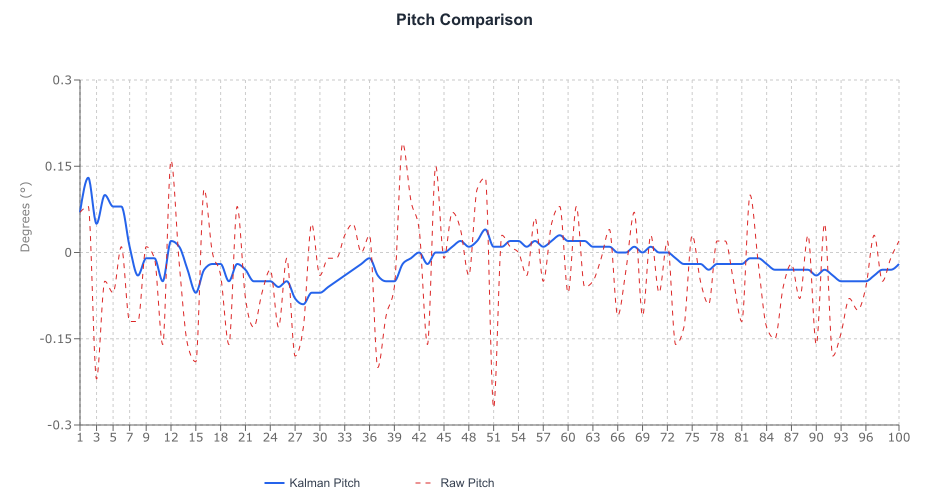
\includegraphics[width=0.8\textwidth]{images/kalman_comparison_pitch_2025-06-23.png}
    \caption{Pitch: Vergleich Rohdaten und Kalman-Filter}
    \label{fig:pitch_pitch}
    \end{figure}

    \begin{figure}[H]
        \centering
        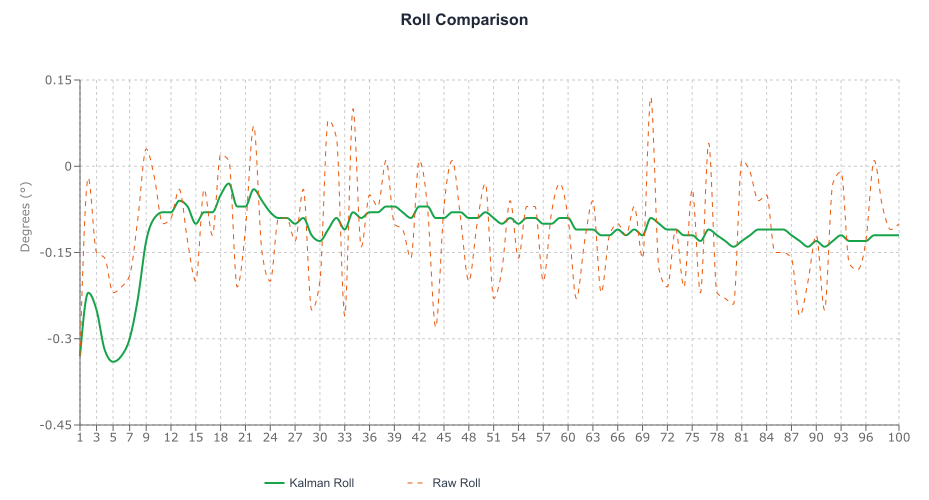
\includegraphics[width=0.8\textwidth]{images/kalman_comparison_roll_2025-06-23.png}
        \caption{Roll: Vergleich Rohdaten und Kalman-Filter}
        \label{fig:roll_roll}
    \end{figure}
\end{samepage}



\section{Gyrosensor Programmierung (Koch)}
Zu Beginn des Projekts war geplant den Gyrosensor MPU6050 zu nutzen, um die Position der Geschützplattform zu bestimmen, da eine kontinuierliche Bewegung um die eigene Achse aufgrund der Kabel nicht möglich ist. Dabei sollte der Sensor über den I2C-Bus mit dem Raspberry Pi 5 verbunden werden, um die Daten auszulesen und zu verarbeiten.
Der MPU6050 ist dabei ein 3-Achsen-Gyroskop und 3-Achsen-Beschleunigungssensor, welcher entsprechende Drehbewegungen und Beschleunigungen entlang der Raumachsen messen kann, welche für eine genaue Winkelbestimmung notwendig sind.

Nach kurzem Einlesen in die Dokumentation waren erste Rohdaten leicht auszulesen. Diese Rohdaten liegen in Form von 16 Bit in zwei Registern bereit und haben die Einheit $\mathit{LSB/g}$ für die Beschleunigungswerte und $\mathit{LSB/^\circ s}$ für die Gyroskop-Werte. Dies gilt es in tatsächliche physikalische Größen umzuwandeln, was bei unserem Projekt letztlich einem Winkel entspricht. 
Um die Beschleunigungswerte nutzen zu können, muss dafür mittels des Skalierungsfaktors die Fallbeschleunigung $\mathit{g}$ errechnet werden, indem man den erhaltenen Wert $x/16384$ rechnet. Die $16384$ ergeben sich aus der Dokumentation und entsprechen den LSB bei einem Messbereich von $\pm2g$, welches der Standardauflösung entspricht und auch die höchste Auflösung des MPU6050 für ist.
Ähnlich wird nun auch Winkelgeschwindigkeit ($\mathit{^\circ s}$) errechnet. Hierbei beträgt der Teiler standardmäßig $131$. \cite[S. 12-13]{raspberry_invensense_mpu6050_datasheet} 

Nach der Umrechnung der Rohdaten in physikalische Größen können nun die Neigungswinkel (Roll- und Pitch-Winkel) des Sensors berechnet werden. Diese ergeben sich aus der Richtung der Erdbeschleunigung relativ zum Sensor. 

Dazu wird die Erweiterung des Arkustangens genutzt, genauer gesagt die Funktion \texttt{atan2}, da sie im Gegensatz zum gewöhnlichen Arctangens auch die Orientierung in allen vier Quadranten berücksichtigt und somit stabile Winkelwerte über den gesamten Bereich von $-180^\circ$ bis $+180^\circ$ liefert. \cite{raspberry_matlab_atan2}

Die Winkelberechnung erfolgt nach der Formel \ref{eq:norms_to_angle}:

\begin{gather}
    \begin{aligned}
    \varphi_\text{pitch} &= \arctan2\left(a_y,\sqrt{a_x^2 + a_z^2}\right) \cdot \frac{180^\circ}{\pi} \\
    \varphi_\text{roll}  &= \arctan2\left(a_x,\sqrt{a_y^2 + a_z^2}\right) \cdot \frac{180^\circ}{\pi}
    \end{aligned}
    \label{eq:norms_to_angle}
\end{gather}


Hierbei sind $a_x$, $a_y$ und $a_z$ die normierten Beschleunigungswerte in $\mathit{g}$ (berechnet aus den Rohwerten durch Division durch $16384$). 

Die $atan2$-Funktion liefert den Winkel zwischen der positiven $x$-Achse und dem Punkt $(x, y)$ in der Ebene, wodurch Sprünge oder Mehrdeutigkeiten bei $90^\circ$ vermieden werden. \cite{raspberry_matlab_atan2}

Nachdem der Term im Code implementiert wurde, konnte ein starkes Rauschen beobachtet werden, was zunächst auf natürliche Schwankungen des Sensors zurückgeführt wurde, weshalb sich dazu entschieden wurde zuerst einen Komplementärfilter zu implementieren,
welcher allerdings das Problem nur bedingt beheben konnte. Deshalb wurde auch noch der Kalman-Filter ausgetestet, wodurch auch eine starke  Rauschunterdrückung festgestellt werden konnte, doch auch hier zeichnete sich ein überdurchschnittliches Rauschverhalten ab, weshalb der Fehler nicht mehr auf ein natürliches Rauschen zurückzuführen war.
Daraufhin wurde auch ein zweiter MPU6050 getestet, welcher ebenfalls dieses Verhalten aufwies, wodurch klar wurde, dass es sich hierbei um einen Programmierfehler handeln muss. Dieser konnte nach einiger Zeit auch herausgefunden werden und lag an der Interpretation der Rohdaten, 
welche fälschlicherweise als \texttt{int16\_t} statt \texttt{uint16\_t} interpretiert wurden.

Aufgrund der aufgewendeten Zeit für die Implementierung des Kalman-Filters sollte dieser aber trotzdem Anwendung im Projekt finden und wird in \ref{sec:kalman_filter} behandelt.

Wie Eingangs erwähnt, sollte der Gyrosensor MPU6050 genutzt werden, um die Position der Geschützplattform zu bestimmen, wofür der Winkel der Drehung um die eigene Achse benötigt wird. Dabei stellte sich heraus das der MPU6050 für diesen Wert zu einem starken Drift neigt, weshalb empfohlen wird diesen mit einem Magnetometer zu kombinieren \cite[S. 26]{raspberry_invensense_mpu6050_datasheet}.
Zur gleichen Zeit stellte sich heraus, dass diese Funktionalität nicht benötigt wird, da über die Servo-Motoren bereits ein Nullpunkt definiert werden konnte, weshalb der Gyrosensor letztlich nur noch für die Neigung der Geschützplattform genutzt wird, um diese als Debug-Information auf dem Webserver \ref{sec:Webserver} anzuzeigen.

\subsection{Kalman Filter Implementierung (Koch)}
\label{sec:kalman_filter}
Der Kalman-Filter ist ein Algorithmus zur Schätzung des Zustands eines dynamischen Systems. Er nutzt Messwerte mit einem mathematischen Modell, um aus verrauschten Daten optimale Schätzungen zu erzeugen und zu filtern, was insbesondere bei Sensoren mit Rauschen, wie dem MPU6050, von Bedeutung ist \cite{raspberry_rwth_kalman_2025}.
Die Berechnung des Kalman-Filters erfolgt nun mittels der Werte des Gyroskops, einer Zeitdifferenz und der zuvor berechneten Roll-und Pitchwinkel. Die Neigungswinkel liefern eine absolute Orientierung relativ zur Erdgravitation, sind jedoch anfällig gegenüber Rauschen und dynamischen Bewegungen, da sie auf Momentanwerten basieren, weshalb man hier auf die Gyroskopwerte zurückgreift.
Diese liefern die Winkelgeschwindigkeit, also die Änderungsrate der Orientierung. Diese Werte werden über die Zeit integriert, um eine relative Winkelschätzung zu erhalten. Sie zeichnen sich durch hohe Kurzzeitstabilität und geringe Reaktionsverzögerung aus, unterliegen jedoch einem Driftverhalten aufgrund von Messabweichungen und systematischen Fehlern.
Der Kalmanfilter fusioniert nun diese beiden Quellen und dessen Vorteile in Relation zum letzten bekannten Zustand.

Dabei besteht der Kalman-Filter aus zwei Hauptphasen: dem Vorhersageschritt (Prediction) und dem Aktualisierungsschritt (Update). Im Vorhersageschritt wird der neue Winkel $\hat{\theta}_{\text{new}}$ basierend auf dem vorherigen Winkel $\hat{\theta}_{\text{prev}}$ und der aktuellen korrigierten Gyroskoprate $\omega$ geschätzt:

\begin{equation*}
\omega = \text{newGyroRate} - \text{bias}, \quad \hat{\theta}_{\text{new}} = \hat{\theta}_{\text{prev}} + dt \cdot \omega
\end{equation*}

Zusätzlich wird die Unsicherheit dieser Vorhersage, dargestellt durch die Kovarianzmatrix $P$, angepasst. Dabei werden sowohl das Zeitintervall $dt$ als auch Modellunsicherheiten, wie der Drift des Gyroskops, berücksichtigt.

Im Aktualisierungsschritt wird der berechnete Winkel $\theta_{\text{meas}}$, welcher mithilfe der Beschleunigungswerte berechnet wurde, mit der Vorhersage verglichen. Die Differenz

\begin{equation*}
S = \theta_{\text{meas}} - \hat{\theta}_{\text{prior}}
\end{equation*}

wird als \emph{Innovation} bezeichnet und wird benötigt um den Kalman-Gain $K$ zu bestimmen. Der Kalman-Gain bestimmt, wie stark diese neue Information zur Korrektur verwendet wird. Er wird aus dem Verhältnis von Unsicherheits-Kovarianzmatrix $P$ und der Innovation $S$ berechnet:

\begin{equation*}
K_0 = \frac{P_{00}}{S}, \quad K_1 = \frac{P_{10}}{S}
\end{equation*}

Hierbei steht $P_{00}$ für die Unsicherheit in der Winkelschätzung, und $P_{10}$ beschreibt die Kovarianz zwischen Winkel und Bias des Gyroskops.

Ein höherer Wert von $K$ bedeutet, dass der Filter der neuen Messung mehr vertraut und ein niedriger Wert zeigt, dass die eigene Vorhersage als zuverlässiger eingeschätzt wird.

Abschließend wird die Kovarianzmatrix $P$ angepasst, um die reduzierte Unsicherheit nach der Messung zu reflektieren. Dadurch wird der Filter präziser in seiner nächsten Schätzung \cite{raspberry_tkjelectronics_kalman_filter_2012}.

Insgesamt erlaubt dieser Algorithmus eine robuste und gleitende Fusion der Sensordaten, wobei kurzfristige Genauigkeit des Gyroskops und langfristige Stabilität des Beschleunigungssensors optimal kombiniert werden.

\begin{samepage}
    In der Abbildung \ref{fig:pitch_pitch} und \ref{fig:roll_roll} ist sowohl für den Pitch, als auch den Roll ein signifikanter Unterschied zwischen den Rohdaten und den gefilterten Daten zu erkennen. Die ersten Schwankungen der gefilterten Werte sind vermutlich genau darauf zurückzuführen, dass der Kalmanfilter mit wenigen Schätzungen noch keinen stabilen Werte für die Kovarianzmatrix und den Bias berechnen konnte, weshalb die Schätzungen auch erst mit steigender Anzahl an Werten genauer werden.
    Der Pitch konnte mithilfe des Kalmanfilters eine Rauschreduktion von $59.4\%$ erzielen und für den Roll $37.4\%$ bei jeweils $100$ Testwerten.

    Aufgrund der Art wie der Gyrosensor auf dem Geschützarm montiert ist, ist für die Neigung allerdings nur der Roll-Wert von Bedeutung.

   \begin{figure}[H]
    \centering
    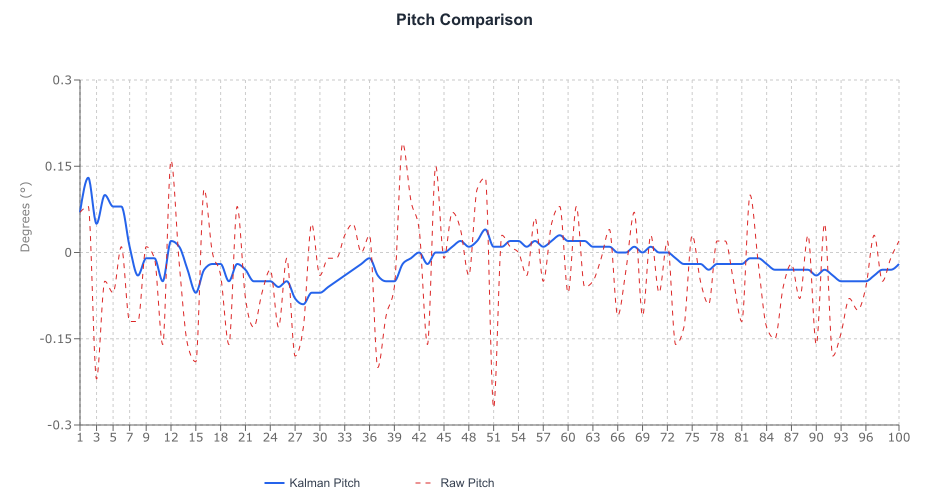
\includegraphics[width=0.8\textwidth]{images/kalman_comparison_pitch_2025-06-23.png}
    \caption{Pitch: Vergleich Rohdaten und Kalman-Filter}
    \label{fig:pitch_pitch}
    \end{figure}

    \begin{figure}[H]
        \centering
        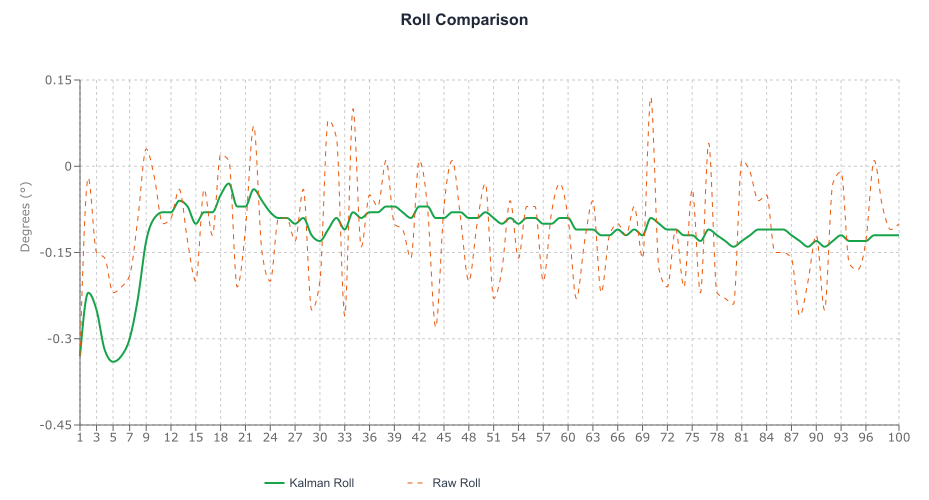
\includegraphics[width=0.8\textwidth]{images/kalman_comparison_roll_2025-06-23.png}
        \caption{Roll: Vergleich Rohdaten und Kalman-Filter}
        \label{fig:roll_roll}
    \end{figure}
\end{samepage}




\chapter{Webserver (Koch)}
\label{sec:Webserver}
\section{Funktion und Anforderung des Webservers}
Der Webserver des Projekts sollte die zentrale Schnittstelle zwischen verschiedenen Sensoren werden und sowohl Videomaterial mit bereits verarbeiteten KI-Informationen darstellen können und wissenswerte Daten wie die Entfernung des Fliegers oder die Geschützneigung anzeigen.
Als zentrales Problem stand dabei das Videomaterial mit entsprechenden Bounding Boxes anzuzeigen im Vordergrund, da bereits über das ganze Projekt hinweg die KI die leistungsintensivste Aufgabe war und entsprechende Latenzprobleme bereits auf das Minimum verringert wurden.
Der Grundlegende Aufbau der KI-Verarbeitung mitsamt der Videoausgabe ist in \ref{JENDRIK} erklärt.

\section{Lösungsansatz und Umsetzung}
Ein Lösungsansatz diesbezüglich war deshalb, dass die Sensordaten vom Raspberry Pi per MQTT an den PC geschickt werden, welcher die KI-Verarbeitung übernimmt, um die Daten direkt im Videostream abzubilden.
Das Video mit den Bounding Boxes und den Sensordaten sollte dann zurück auf den MediaMTX-Server geschickt werden, worüber man dann das Video sehen kann.
Dieser Ansatz war allerdings keine geeignete Lösung, da die Verarbeitung zu lange dauerte und somit eine zu geringe Framerate erreicht wurde, wodurch dies keine annehmbare Lösung darstellte.


Deshalb wurde der alternative Ansatz gewählt, dass der Raspberry Pi selbst den Webserver bereitstellt, da dieser bereits die Sensordaten und den MediaMTX-Server bereitstellt.
Das Problem hierbei war jedoch, dass somit zwar der Videostream und die Sensordaten dargestellt werden konnten, allerdings noch keine Bounding Boxes, welche eine harte Anforderung an den Webserver waren.
Es musste also eine Lösung gefunden werden, den verarbeiteten Videostream mit den Bounding Boxes vom PC zum Raspberry Pi zu übertragen, doch das senden des Videostreams ist nicht ohne Verluste möglich, wie bereits erwähnt wurde.

Die Umsetzung erfolgte über einen zentralen Knotenpunkt auf dem Raspberry Pi, welcher sowohl die Bereitstellung der Benutzeroberfläche als auch die Echtzeitkommunikation mit den Sensoren und der externen KI-Komponente zur Objekterkennung übernimmt. Die Kommunikation erfolgt über WebSockets, wobei sowohl Sensordaten als auch Bounding-Box-Koordinaten empfangen, verarbeitet und an das Frontend weitergeleitet werden. Die Darstellung im Browser kombiniert dabei Livevideo, Sensordaten und erkannte Objekte in einem einheitlichen Interface. 
Dabei wird die Entfernung nur in Kombination mit der Bounding Box ausgegeben wie in Abbildung \ref{fig:webserver} zu sehen.
Während der Entwicklung zeigte sich, dass die zunächst gewählte Architektur zur Sensoranbindung zu erheblichen Verzögerungen führte. Die ursprüngliche Implementierung versuchte, beide Sensoren (Gyrosensor und Ultraschallsensor) über asynchrone Generatoren auszulesen, jedoch geschah dies nur sequentiell. Vermutlich bremste dabei die Verarbeitung des Ultraschallsensors, der mit geringerer Frequenz Daten liefert, die Verarbeitung des Gyrosensors aus. In der Folge wurden die Gyroskopdaten gepuffert und verzögert ausgegeben.
Um dieses Problem zu beheben, wurde die Architektur angepasst und die Sensorverarbeitung parallelisiert. Statt beide Generatoren sequentiell abzufragen, wurden zwei Tasks erstellt, die jeweils eigenständig mit ihrem Sensor kommunizieren. Dadurch können beide Datenströme unabhängig voneinander verarbeitet und weitergeleitet werden, was die Reaktionszeit des Systems verbesserte und die gleichzeitige Darstellung der Sensorinformationen im Frontend ermöglichte.
\begin{figure}[H]
    \begin{center}
        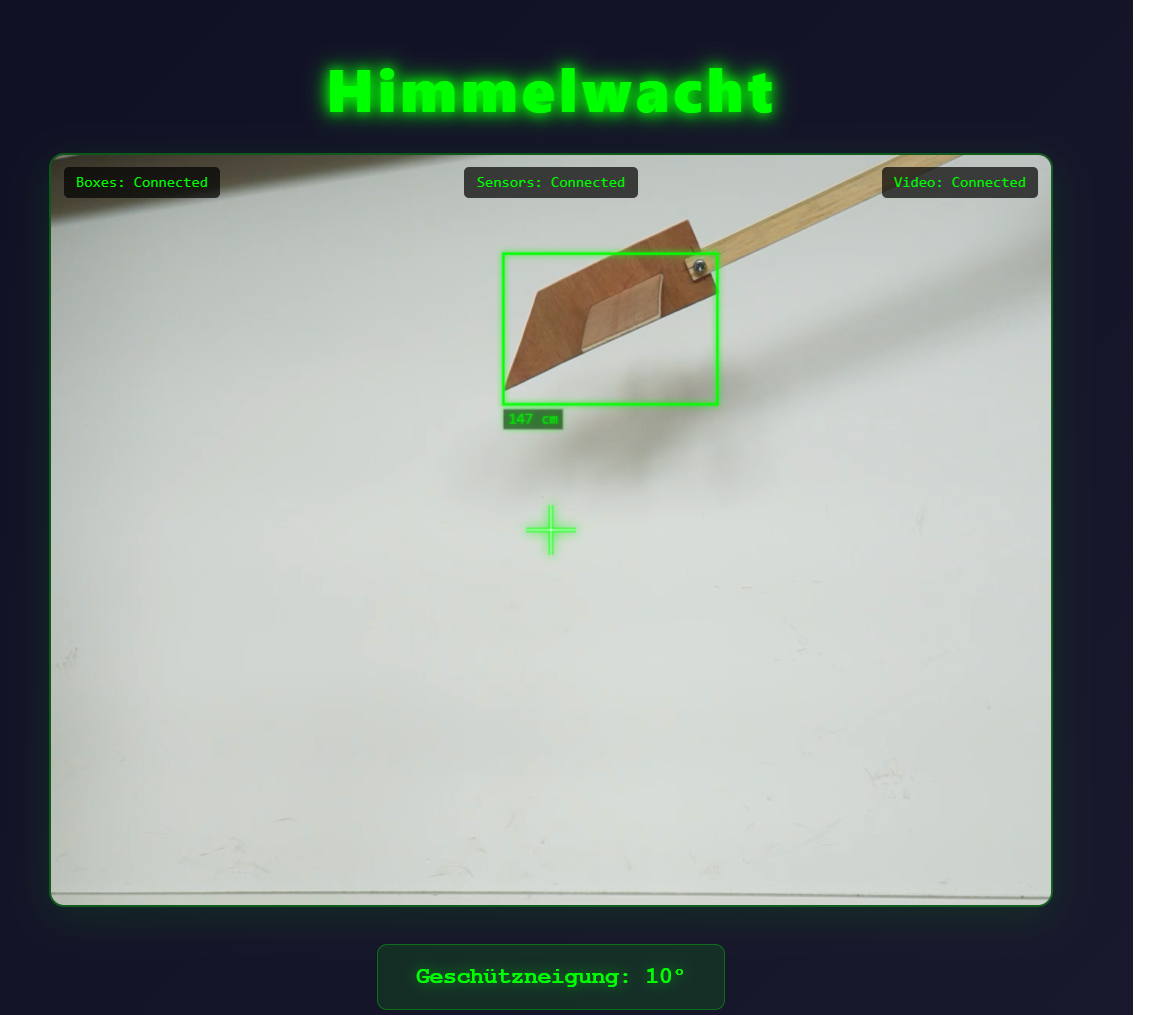
\includegraphics[width=0.8\textwidth]{images/Webserver.png}
        \caption{Webinterface zur Darstellung des Videostreams mit Bounding Boxes und Sensordaten}
        \label{fig:webserver}
    \end{center}
\end{figure}
%\input{gnn}
%\input{p5p}
%\input{end.tex}

% Time tables
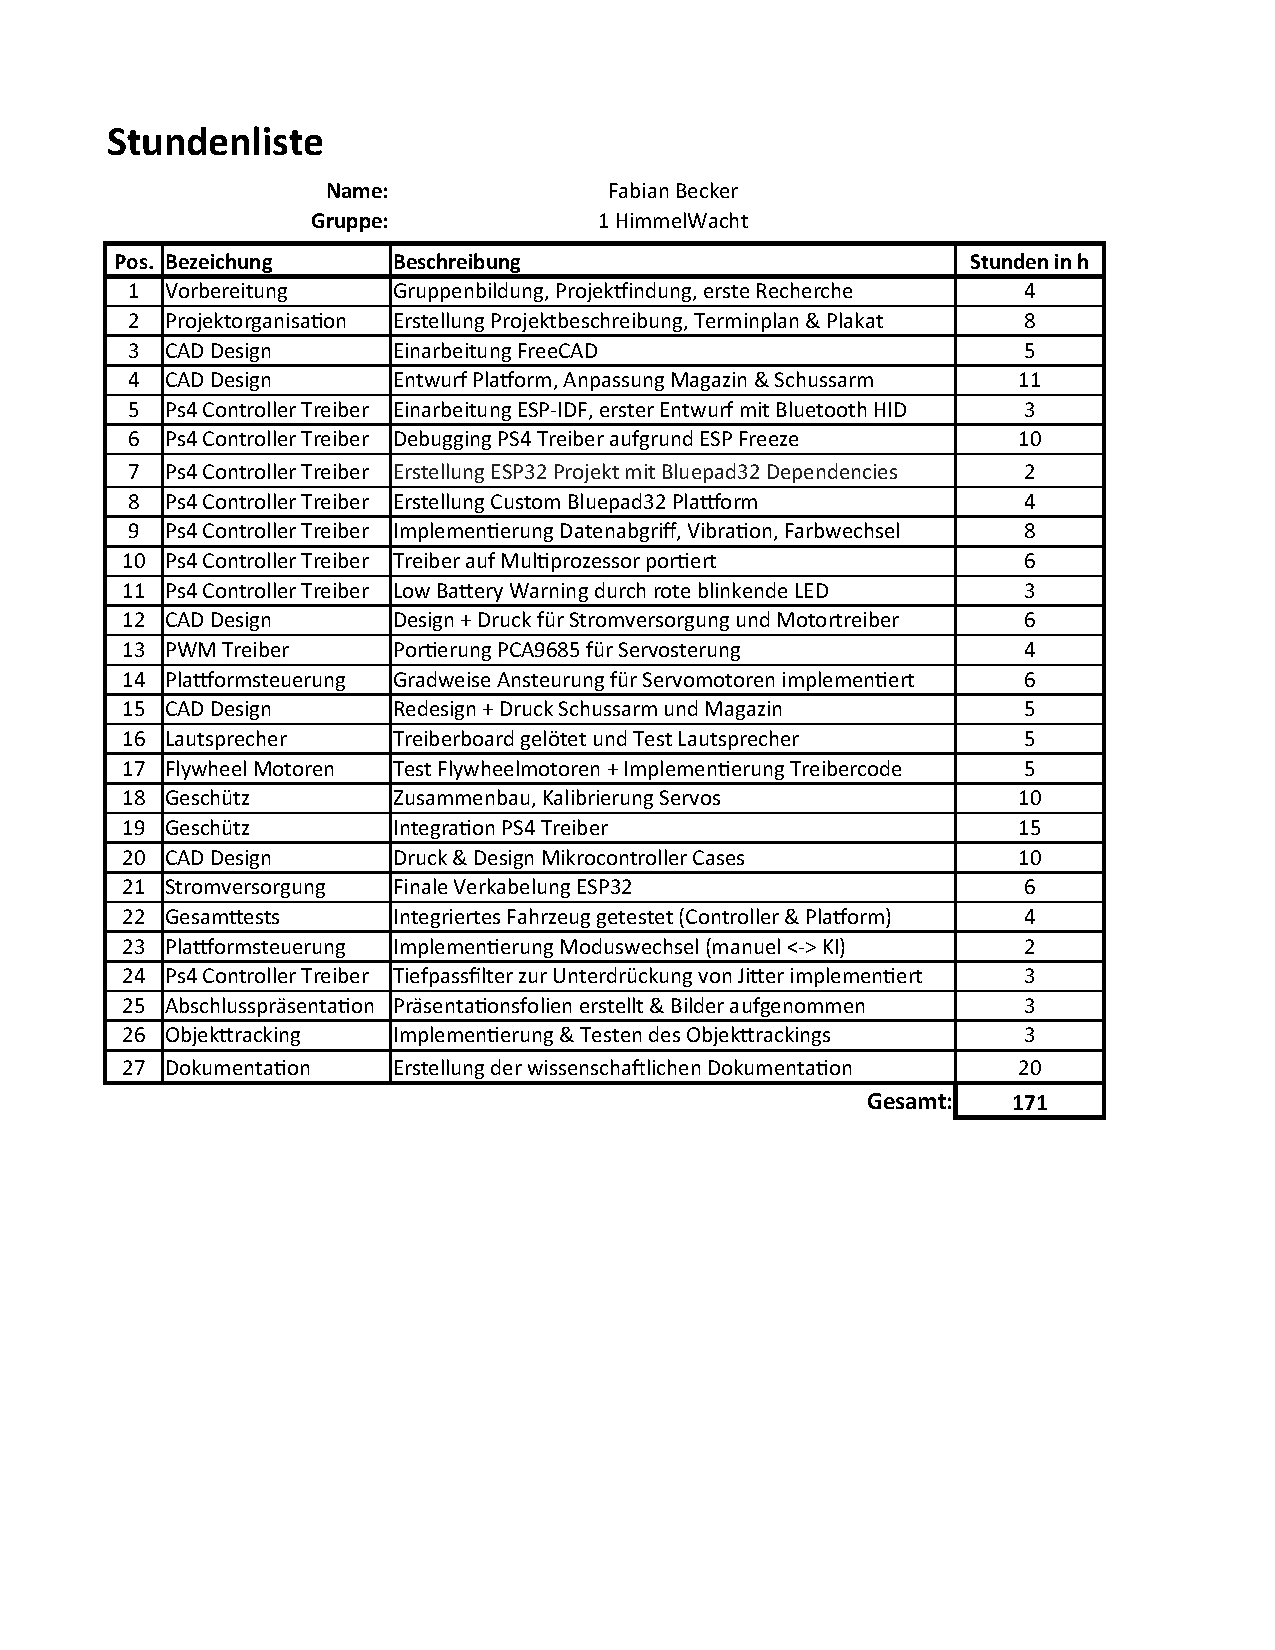
\includepdf[pages=-]{pdfs/Stundenliste_Fabian_Becker.pdf}
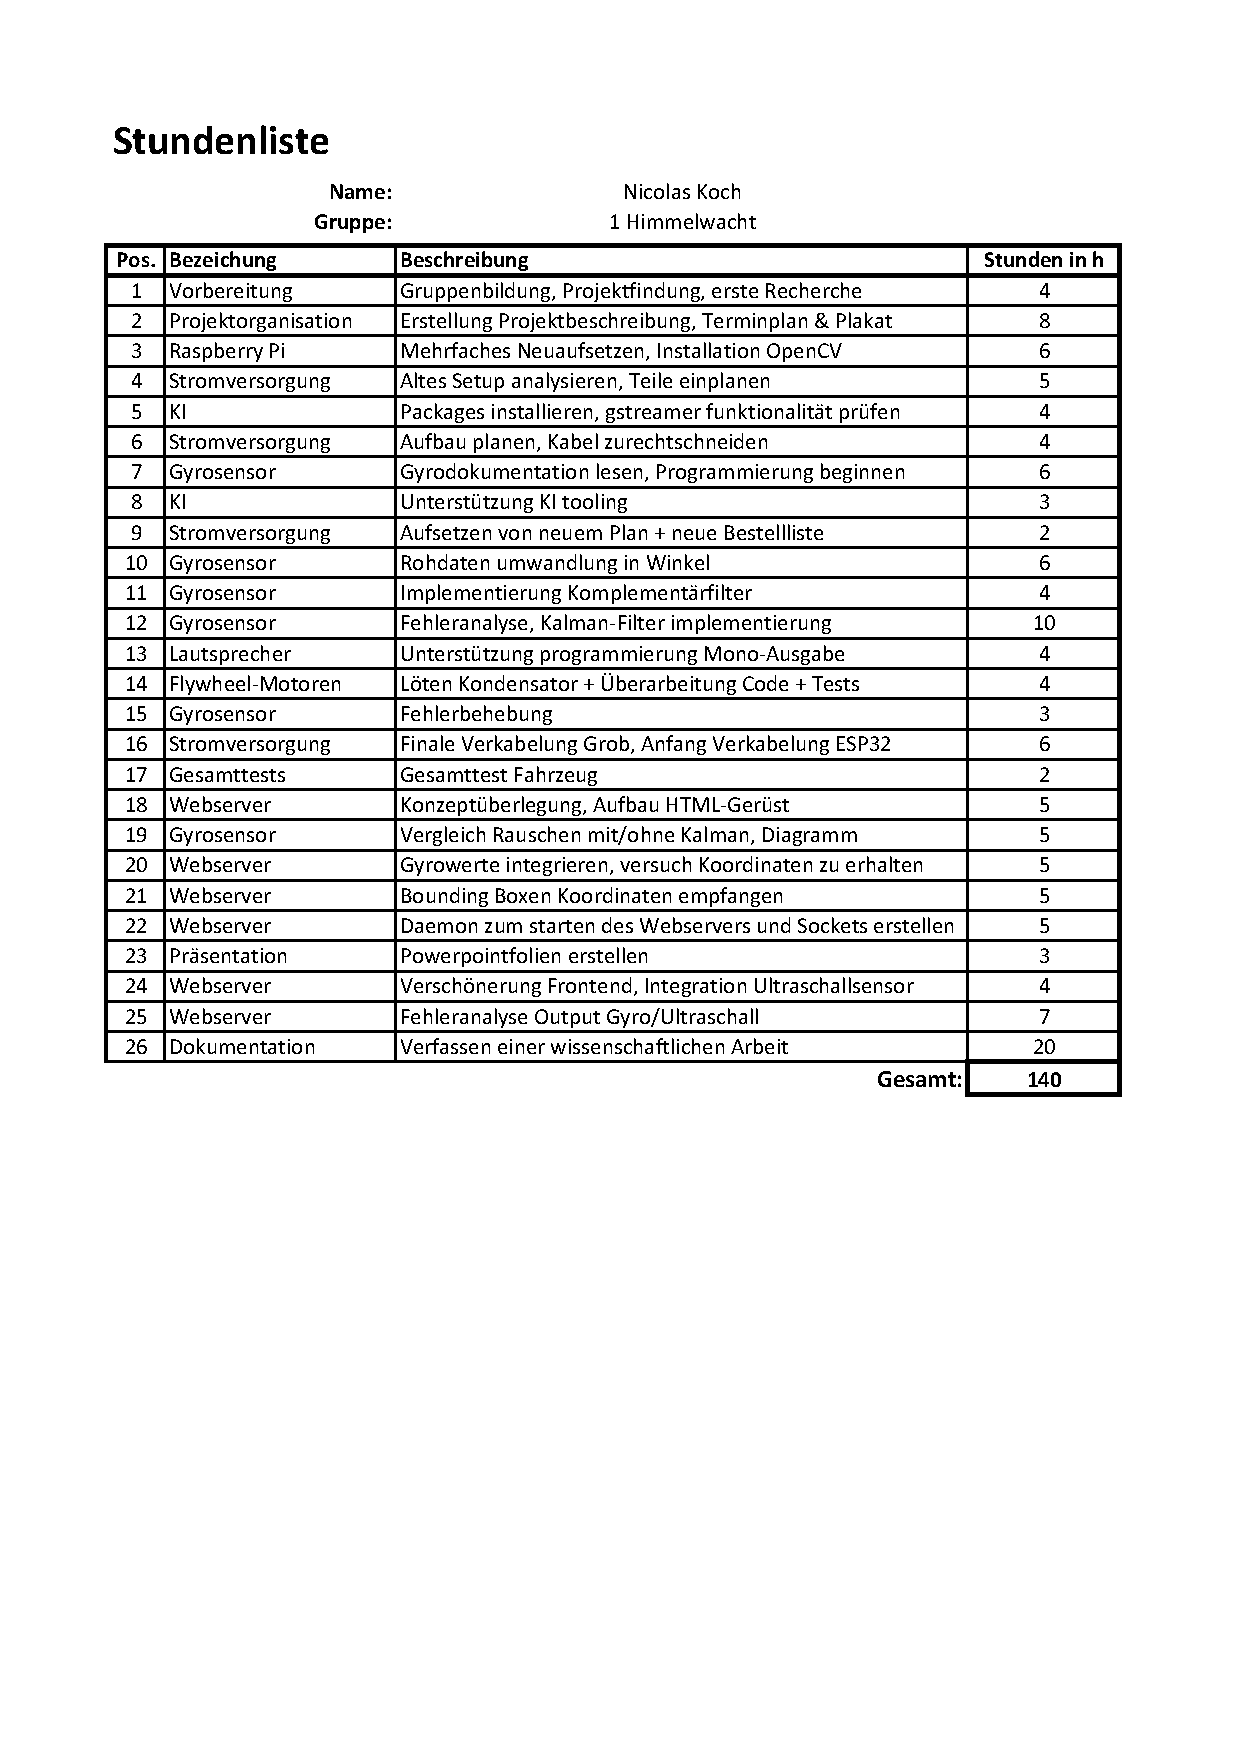
\includepdf[pages=-]{pdfs/Stundenliste_Nicolas_Koch.pdf}
% \includepdf[pages=-]{Stundenliste_Jendrik_Jürgens.pdf}
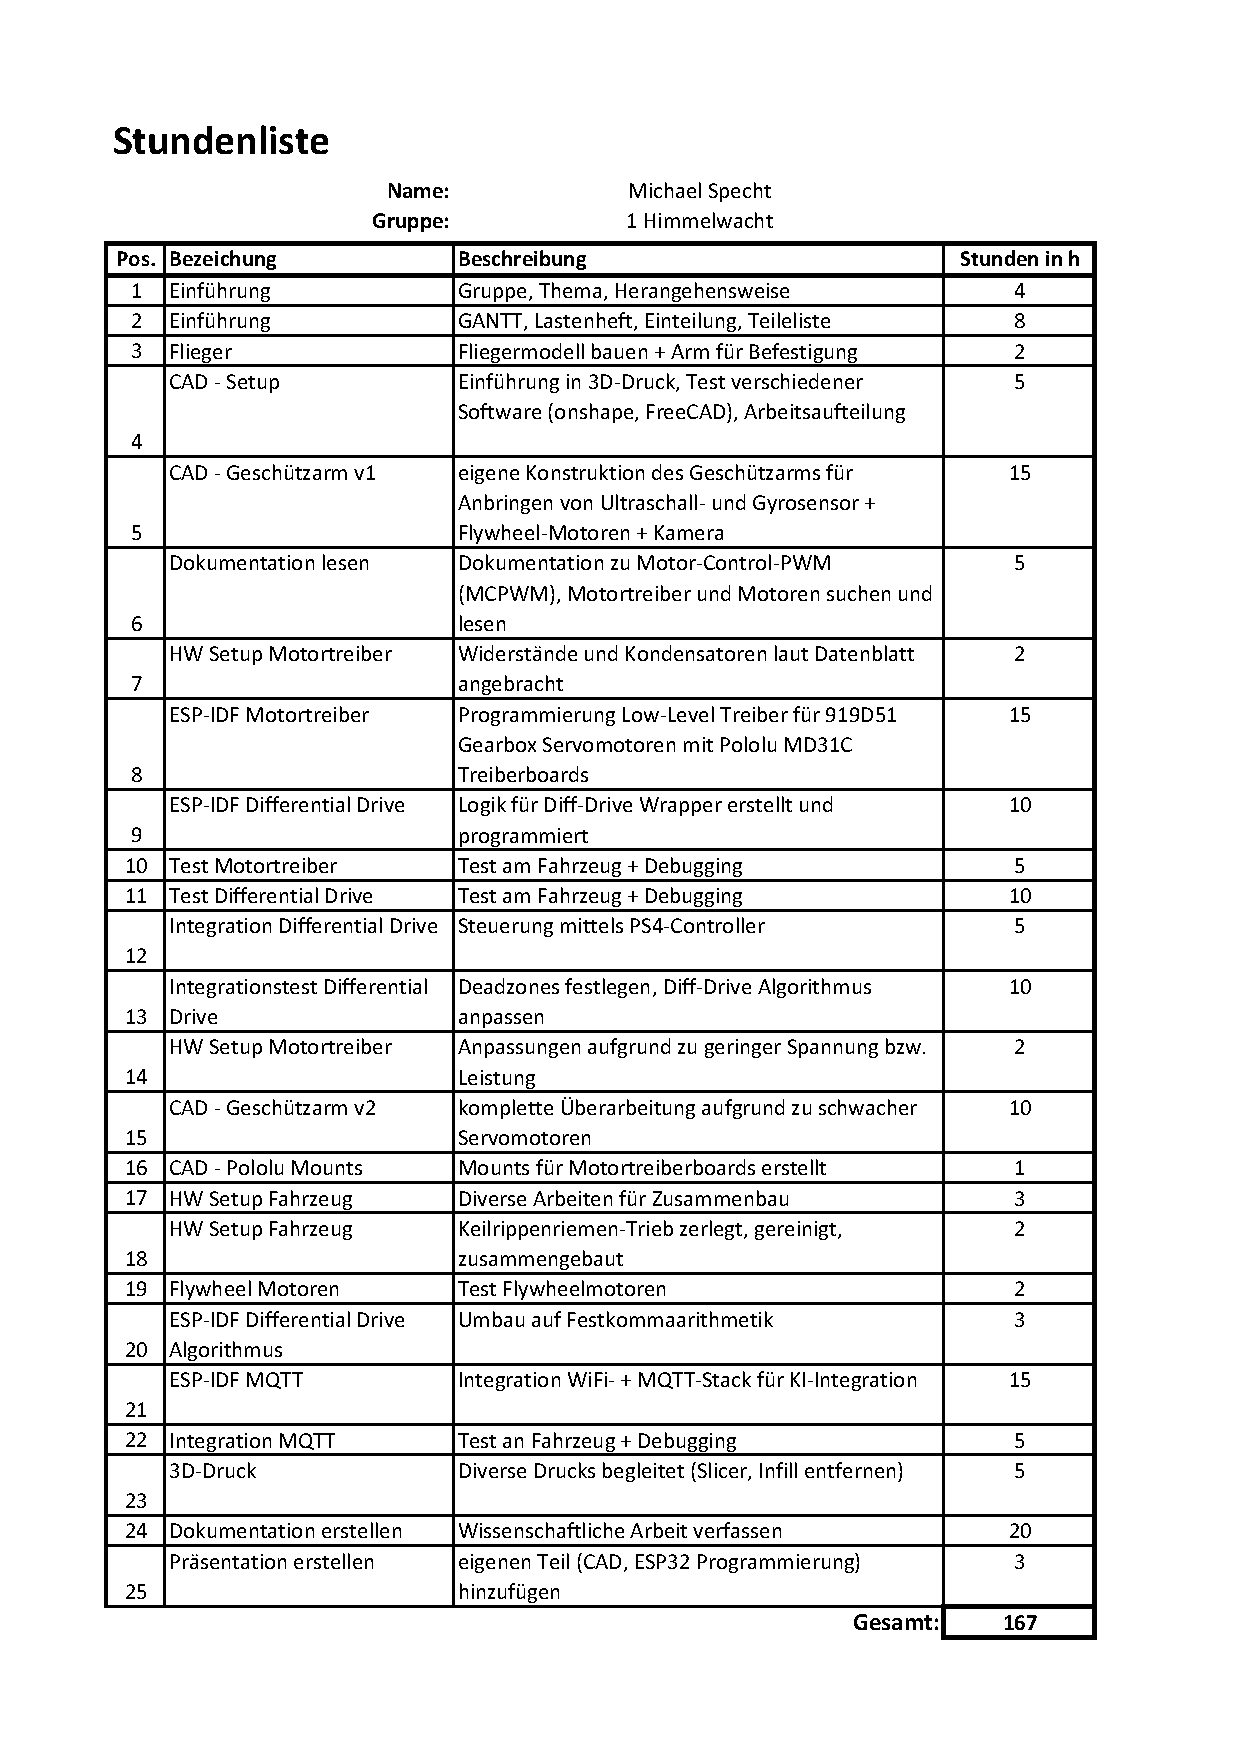
\includepdf[pages=-]{pdfs/Stundenliste_Michael_Specht.pdf}
% 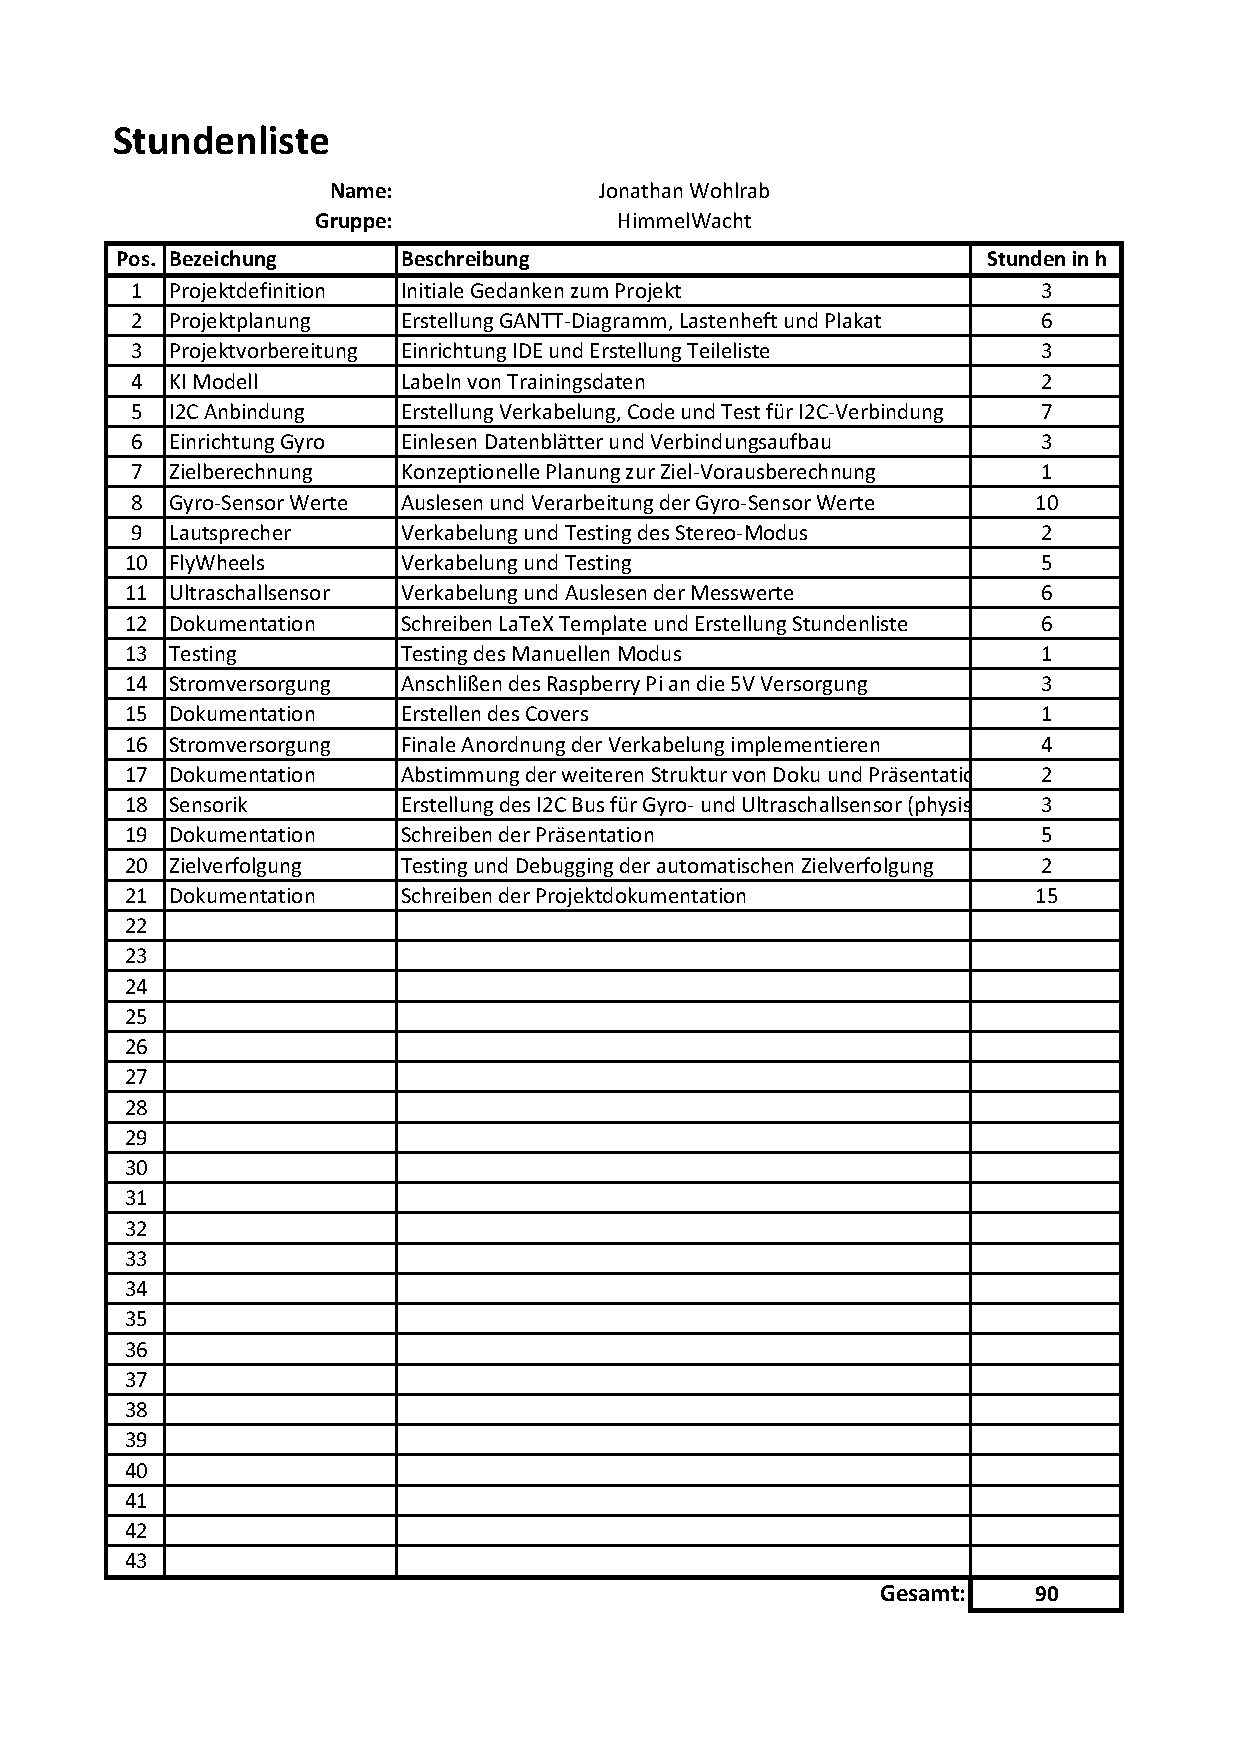
\includepdf[pages=-]{Stundenliste_Jonathan_Wohlrab.pdf}

% List of Figures
\listoffigures
\addcontentsline{toc}{chapter}{Abbildungsverzeichnis}
\newpage

% List of Tables
\listoftables
\addcontentsline{toc}{chapter}{Tabellenverzeichnis}
\newpage

% List of Acronyms
%\addcontentsline{toc}{chapter}{Abkürzungen}
% \printacronyms[heading=chapter*]
%\newpage

% Bibliography
\newpage
\begin{sloppypar}
  \addcontentsline{toc}{chapter}{Literaturverzeichnis} % Add to ToC
  \printbibliography[title=Literaturverzeichnis]
\end{sloppypar}

% Annex
% \input{annex.tex}

\end{document}
